\documentclass[11pt]{article}
\usepackage{graphicx}
\pagestyle{myheadings}

%------------------------------------------------------------------------------
\newcommand{\stardoccategory}  {Starlink User Note}
\newcommand{\stardocinitials}  {SUN}
\newcommand{\stardocsource}    {sun85.6}
\newcommand{\stardocnumber}    {85.6}
\newcommand{\stardocauthors}   {P T Wallace \& D L Terrett}
\newcommand{\stardocdate}      {10 July 1995}
\newcommand{\stardoctitle}     {SGS --- Simple Graphics System}
%------------------------------------------------------------------------------

\newcommand{\stardocname}{\stardocinitials /\stardocnumber}
\markright{\stardocname}
\setlength{\textwidth}{160mm}
\setlength{\textheight}{230mm}
\setlength{\topmargin}{-2mm}
\setlength{\oddsidemargin}{0mm}
\setlength{\evensidemargin}{0mm}
\setlength{\parindent}{0mm}
\setlength{\parskip}{\medskipamount}
\setlength{\unitlength}{1mm}

% -----------------------------------------------------------------------------
% Hypertext definitions.
% These are used by the LaTeX2HTML translator in conjuction with star2html.

% Comment.sty: version 2.0, 19 June 1992
% Selectively in/exclude pieces of text.
%
% Author
%    Victor Eijkhout                                      <eijkhout@cs.utk.edu>
%    Department of Computer Science
%    University Tennessee at Knoxville
%    104 Ayres Hall
%    Knoxville, TN 37996
%    USA

%  Do not remove the %begin{latexonly} and %end{latexonly} lines (used by
%  star2html to signify raw TeX that latex2html cannot process).
%begin{latexonly}
\makeatletter
\def\makeinnocent#1{\catcode`#1=12 }
\def\csarg#1#2{\expandafter#1\csname#2\endcsname}

\def\ThrowAwayComment#1{\begingroup
    \def\CurrentComment{#1}%
    \let\do\makeinnocent \dospecials
    \makeinnocent\^^L% and whatever other special cases
    \endlinechar`\^^M \catcode`\^^M=12 \xComment}
{\catcode`\^^M=12 \endlinechar=-1 %
 \gdef\xComment#1^^M{\def\test{#1}
      \csarg\ifx{PlainEnd\CurrentComment Test}\test
          \let\html@next\endgroup
      \else \csarg\ifx{LaLaEnd\CurrentComment Test}\test
            \edef\html@next{\endgroup\noexpand\end{\CurrentComment}}
      \else \let\html@next\xComment
      \fi \fi \html@next}
}
\makeatother

\def\includecomment
 #1{\expandafter\def\csname#1\endcsname{}%
    \expandafter\def\csname end#1\endcsname{}}
\def\excludecomment
 #1{\expandafter\def\csname#1\endcsname{\ThrowAwayComment{#1}}%
    {\escapechar=-1\relax
     \csarg\xdef{PlainEnd#1Test}{\string\\end#1}%
     \csarg\xdef{LaLaEnd#1Test}{\string\\end\string\{#1\string\}}%
    }}

%  Define environments that ignore their contents.
\excludecomment{comment}
\excludecomment{rawhtml}
\excludecomment{htmlonly}

%  Hypertext commands etc. This is a condensed version of the html.sty
%  file supplied with LaTeX2HTML by: Nikos Drakos <nikos@cbl.leeds.ac.uk> &
%  Jelle van Zeijl <jvzeijl@isou17.estec.esa.nl>. The LaTeX2HTML documentation
%  should be consulted about all commands (and the environments defined above)
%  except \xref and \xlabel which are Starlink specific.

\newcommand{\htmladdnormallinkfoot}[2]{#1\footnote{#2}}
\newcommand{\htmladdnormallink}[2]{#1}
\newcommand{\htmladdimg}[1]{}
\newenvironment{latexonly}{}{}
\newcommand{\hyperref}[4]{#2\ref{#4}#3}
\newcommand{\htmlref}[2]{#1}
\newcommand{\htmlimage}[1]{}
\newcommand{\htmladdtonavigation}[1]{}
\newcommand{\latexhtml}[2]{#1}
\newcommand{\html}[1]{}

% Starlink cross-references and labels.
\newcommand{\xref}[3]{#1}
\newcommand{\xlabel}[1]{}

%  LaTeX2HTML symbol.
\newcommand{\latextohtml}{{\bf LaTeX}{2}{\tt{HTML}}}

%  Define command to recentre underscore for Latex and leave as normal
%  for HTML (severe problems with \_ in tabbing environments and \_\_
%  generally otherwise).
\newcommand{\latex}[1]{#1}
\newcommand{\setunderscore}{\renewcommand{\_}{{\tt\symbol{95}}}}
\latex{\setunderscore}

% -----------------------------------------------------------------------------
%  Debugging.
%  =========
%  Un-comment the following to debug links in the HTML version using Latex.

% \newcommand{\hotlink}[2]{\fbox{\begin{tabular}[t]{@{}c@{}}#1\\\hline{\footnotesize #2}\end{tabular}}}
% \renewcommand{\htmladdnormallinkfoot}[2]{\hotlink{#1}{#2}}
% \renewcommand{\htmladdnormallink}[2]{\hotlink{#1}{#2}}
% \renewcommand{\hyperref}[4]{\hotlink{#1}{\S\ref{#4}}}
% \renewcommand{\htmlref}[2]{\hotlink{#1}{\S\ref{#2}}}
% \renewcommand{\xref}[3]{\hotlink{#1}{#2 -- #3}}{}
%end{latexonly}
% -----------------------------------------------------------------------------
% Add any document specific \newcommand or \newenvironment commands here
\newcommand{\routinehead}[1]{\vspace{\bigskipamount}{\large\bf#1}}
\newenvironment{routinelist}{\begin{list}{}{\setlength{\leftmargin}{2cm}
                             \setlength{\parsep}{\smallskipamount}}}{\end{list}}
\newcommand{\routine}[2]{\item\hspace{-1cm}#1#2\\}

\begin{htmlonly}
  \newcommand{\routinehead}[1]{\subsection{#1}}
  \newcommand{\routine}[2]{\item \htmlref{#1}{#1}#2\\}
\end{htmlonly}

\newcommand{\rthead}[2]{\rule{\textwidth}{0.3mm}
{\Large {\bf #1} \hfill #2 \hfill {\bf #1}}}
\newenvironment{params}%
{\[\begin{tabular}{p{0.14\textwidth}p{0.05\textwidth}p{0.66\textwidth}}}%
{\end{tabular}\]}
\newcommand{\rparams}[3]{{\em #1} &#2 &#3\\}

\begin{htmlonly}
  \newcommand{\rthead}[2]{\subsection{\label{#1}\xlabel{#1}#1 - #2}}
  \newenvironment{params}{\begin{description}}{\end{description}}
  \newcommand{\rparams}[3]{\item{{\em #1}} (#2) #3}
\end{htmlonly}


% -----------------------------------------------------------------------------
%  Title Page.
%  ===========
\begin{document}
\thispagestyle{empty}

%  Latex document header.
\begin{latexonly}
   CCLRC / {\sc Rutherford Appleton Laboratory} \hfill {\bf \stardocname}\\
   {\large Particle Physics \& Astronomy Research Council}\\
   {\large Starlink Project\\}
   {\large \stardoccategory\ \stardocnumber}
   \begin{flushright}
   \stardocauthors\\
   \stardocdate
   \end{flushright}
   \vspace{-4mm}
   \rule{\textwidth}{0.5mm}
   \vspace{5mm}
   \begin{center}
   {\Large\bf \stardoctitle}
   \end{center}
   \vspace{5mm}

%  Add heading for abstract if used.
%   \vspace{10mm}
%   \begin{center}
%      {\Large\bf Description}
%   \end{center}
\end{latexonly}

%  HTML documentation header.
\begin{htmlonly}
   \xlabel{}
   \begin{rawhtml} <H1> \end{rawhtml}
      \stardoctitle
   \begin{rawhtml} </H1> \end{rawhtml}

%  Add picture here if required.

   \begin{rawhtml} <P> <I> \end{rawhtml}
   \stardoccategory\ \stardocnumber \\
   \stardocauthors \\
   \stardocdate
   \begin{rawhtml} </I> </P> <H3> \end{rawhtml}
      \htmladdnormallink{CCLRC}{http://www.clrc.ac.uk} /
      \htmladdnormallink{Rutherford Appleton Laboratory}
                        {http://www.clrc.ac.uk/ral} \\
      Particle Physics \& Astronomy Research Council \\
   \begin{rawhtml} </H3> <H2> \end{rawhtml}
      \htmladdnormallink{Starlink Project}{http://www.starlink.ac.uk/}
   \begin{rawhtml} </H2> \end{rawhtml}
   \htmladdnormallink{\htmladdimg{source.gif} Retrieve hardcopy}
      {http://www.starlink.ac.uk/cgi-bin/hcserver?\stardocsource}\\

%  Start new section for abstract if used.
%  \section{\xlabel{abstract}Abstract}

\end{htmlonly}

% -----------------------------------------------------------------------------
%  Document Abstract. (if used)
%  ==================
% -----------------------------------------------------------------------------
%  Table of Contents. (if used)
%  ==================
%  The commands used here disable the creation of a "second" table of
%  contents and create a button in the navigation panel to get to the
%  postion of the \label{stardoccontents} command. If this isn't the
%  behaviour you require remove the htmlonly environment (and its
%  contents) and the \begin{latexonly} and \end{latexonly}.
%
% \begin{htmlonly}
%    \htmladdtonavigation{\htmlref{\htmladdimg{contents_motif.gif}}
%                                             {stardoccontents}}
%   \label{stardoccontents}
%   \begin{rawhtml}
%      <HR>
%      <H2>Contents</H2>
%   \end{rawhtml}
% \end{htmlonly}
% \begin{latexonly}
%    \setlength{\parskip}{0mm}
%    \tableofcontents
%    \setlength{\parskip}{\medskipamount}
%    \markright{\stardocname}
% \end{latexonly}
% -----------------------------------------------------------------------------

\section{INTRODUCTION}

SGS is a set of subroutines for performing low-level graphics input/output.
SGS is implemented above the GKS package (described in \xref{SUN/83}{sun83},
the RAL GKS Guide
and the ISO document GKS 7.4) which is a device independent graphics system
designed to be the kernel of a wide variety of graphics systems.
GKS, which is very comprehensive, does not itself set out to provide the most
convenient interfaces for all applications, and SGS allows easy access to many
of its more straightforward features.

SGS, while preserving GKS concepts and indeed allowing direct GKS calls to be
interspersed with SGS calls, is optimised for convenience in simple cases.
Many of its features are low level (for example: open, draw a line, draw a text
string, close), but there are some routines of a slightly higher level (drawing
arcs and formatted numbers etc).
SGS does not include routines for high level operations like drawing annotated
axes or complete graphs.

Many plotting programs will be written entirely with SGS or higher level calls.
There will, however, be occasions when GKS routines are used as well, usually
because a specialised feature of GKS is needed. Therefore this user manual uses
GKS concepts to describe SGS, and
\hyperref{this appendix}{Appendix~}{}{app-subroutines} describes SGS
routines in terms of their effect on GKS. This will allow programmers to mix
GKS and SGS calls in safety. The unadventurous user may safely ignore the
appendices.

Throughout this manual the normal FORTRAN variable naming conventions are
adhered to:  i.e.\ all integers start with the letters I--N, all reals with
letters A--H and O--Z. Character and logical variables have their type
explicitly referenced in the text.


\section{SUMMARY OF SGS CALLS}\label{sec-summary}

\routinehead{Control}
\begin{routinelist}
\routine {SGS\_OPEN}{(WKSTN, IZONID, ISTAT)}
   Open SGS \& GKS, opening and activating one workstation.
\routine {SGS\_INIT}{(LUN, ISTAT)}
   Open SGS \& GKS, without opening a workstation.
\routine {SGS\_CLOSE}{}
   Shut down SGS \& GKS.
\routine {SGS\_OPNWK}{(WKSTN, IZONID, ISTAT)}
   Open a new workstation and select it.
\routine {SGS\_CLSWK}{(IZONID, ISTAT)}
   Close a workstation.
\routine {SGS\_WLIST}{(LUN)}
   Output a list of available workstations.
\routine {SGS\_SPEN}{(NPEN)}
   Select pen for line and text drawing.
\routine {SGS\_IPEN}{(NPEN)}
   Inquire current pen number.
\routine {SGS\_FLUSH}{}
   Complete all pending output.
\routine {SGS\_ISLER}{(BLKER)}
   Inquire whether device has selective erase capability.
\routine {SGS\_CLRFG}{(ISTATE)}
   Set or clear `clear display on open' flag.
\end{routinelist}

\routinehead{Zones}
\begin{routinelist}
\routine {SGS\_ZONE}{(X1, X2, Y1, Y2, IZONID, ISTAT)}
   Create and select a zone of the specified extent.
\routine {SGS\_ZSHAP}{(AR, POS, IZONID, ISTAT)}
   Create and select a zone of the specified aspect ratio.
\routine {SGS\_ZSIZE}{(XM, YM, POS, IZONID, ISTAT)}
   Create and select a zone of the specified size.
\routine {SGS\_ZPART}{(NX, NY, IZONES, ISTAT)}
   Partition current zone into NX by NY pieces.
\routine {SGS\_SW}{(X1, X2, Y1, Y2, ISTAT)}
   Set window of current zone to given bounds.
\routine {SGS\_SELZ}{(IZONID, ISTAT)}
   Select another zone.
\routine {SGS\_RELZ}{(IZONID)}
   Release the specified zone.
\routine {SGS\_CLRZ}{}
   Clear the current zone (even if this means clearing the whole display
   surface).
\routine {SGS\_ICURZ}{(IZONID)}
   Inquire ID of current zone.
\routine {SGS\_IZONE}{(X1, X2, Y1, Y2, XM, YM)}
   Inquire window bounds for the current zone, and its size on the display
   surface.
\routine {SGS\_IDUN}{(DXW,DYW)}
   Inquire the plotting resolution of the current zone.
\routine {SGS\_TPZ}{(IZIN, XIN, YIN, IZOUT, XOUT, YOUT, ISTAT)}
   Transform position from one zone to another.
\routine {SGS\_BZNDC}{(X1, X2, Y1, Y2, POS, ISTAT)}
   Set the NDC extent of a base zone.
\end{routinelist}

\routinehead{Plotting Lines}
\begin{routinelist}
\routine {SGS\_BPOLY}{(X, Y)}
   Begin a new polyline.
\routine {SGS\_APOLY}{(X, Y)}
   Append a new line to the polyline.
\routine {SGS\_OPOLY}{}
   Output the polyline.
\routine {SGS\_IPLXY}{(X, Y)}
   Inquire end of current polyline.
\routine {SGS\_LINE}{(X1, Y1, X2, Y2)}
   Begin a new polyline with a single line.
\routine {SGS\_BOX}{(X1, X2, Y1, Y2)}
   Draw a rectangle.
\routine {SGS\_CIRCL}{(X, Y, R)}
   Draw a circle.
\routine {SGS\_ARC}{(X, Y, R, THETA1, THETA2)}
   Draw an arc of a circle.
\routine {SGS\_CLRBL}{(X1, X2, Y1, Y2)}
   Clear a rectangular area (if this can be done without affecting the rest of
   the display surface).
\end{routinelist}

\routinehead{Plotting Text}
\begin{routinelist}
\routine {SGS\_BTEXT}{(X, Y)}
   Begin a new text string.
\routine {SGS\_ATEXT}{(STRING)}
   Append text to the current string.
\routine {SGS\_OTEXT}{}
   Output the text string.
\routine {SGS\_ATXI}{(I, NFI)}
   Format an integer onto the current text string.
\routine {SGS\_ATXR}{(R, NFI, NDP)}
   Format a real number onto the current text string.
\routine {SGS\_ATXL}{(STRING)}
   Append text to the current text string omitting trailing blanks.
\routine {SGS\_ATXB}{(STRING, NSPACE)}
   Append right justified field to the current text string.
\routine {SGS\_TX}{(X, Y, STRING)}
   Begin a new text string with a string.
\routine {SGS\_TXI}{(X, Y, I, NFI)}
   Begin a new text string with a formatted integer.
\routine {SGS\_TXR}{(X, Y, R, NFI, NDP)}
   Begin a new text string with a formatted real number.
\routine {SGS\_ITXB}{(X, Y, N, DX, DY)}
   Inquire status of current text string.
\end{routinelist}

\routinehead{Plotting Markers}
\begin{routinelist}
\routine {SGS\_MARK}{(X, Y, MTYPE)}
   Draw a single marker.
\routine {SGS\_MARKL}{(MTYPE)}
   Draw marker at current end of polyline.
\end{routinelist}

\routinehead{Attributes of Characters}
\begin{routinelist}
\routine {SGS\_SFONT}{(NF)}
   Select text font.
\routine {SGS\_SPREC}{(NPR)}
   Specify text precision.
\routine {SGS\_SHTX}{(HT)}
   Specify character height.
\routine {SGS\_SARTX}{(AR)}
   Specify text aspect ratio.
\routine {SGS\_SUPTX}{(XU, YU)}
   Specify character orientation.
\routine {SGS\_SSPTX}{(SP)}
   Specify character spacing.
\routine {SGS\_STXJ}{(TXJ)}
   Specify text alignment.
\routine {SGS\_ITXA}{(NF, NPR, HT, AR, XU, YU, SP, TXJ)}
   Inquire text attributes.
\end{routinelist}

\routinehead{Input}
\begin{routinelist}
\routine {SGS\_CUVIS}{(VIS)}
   Set visibility of cursor.
\routine {SGS\_DEFCH}{(CHOSTR)}
   Define valid choice keys.
\routine {SGS\_DISCU}{}
   Disable sample mode for cursor.
\routine {SGS\_ENSCU}{}
   Enable sample mode for cursor.
\routine {SGS\_ICUAV}{(AVAIL)}
   Inquire cursor availability.
\routine {SGS\_INCHO}{(NCHDEV, N)}
   Inquire number of choices.
\routine {SGS\_REQCH}{(N)}
   Request choice.
\routine {SGS\_REQCU}{(X, Y, N)}
   Request cursor position.
\routine {SGS\_SAMCU}{(X, Y)}
   Sample cursor position.
\routine {SGS\_SELCH}{(NCHDEV)}
   Select choice device.
\routine {SGS\_SETCU}{(X, Y)}
   Set cursor position.
\end{routinelist}

\routinehead{GKS Inquiries} (described in
\hyperref{this appendix}{Appendix~}{}{app-interaction})
\begin{routinelist}
\routine {SGS\_ICURW}{(IWKID)}
   Inquire workstation ID for the current zone.
\routine {SGS\_WIDEN}{(WKSTN, IWTYPE, ICONID, ISTAT)}
   Translate workstation name to GKS type and connection ID.
\routine {SGS\_WNAME}{(ROUTIN, I, ISTAT)}
   Get list of workstation names.
\end{routinelist}

\section {CONTROL FUNCTIONS}\label{sec-control}

\subsection {Opening and closing SGS \& GKS}\label{sec-op-cl}

\begin{quote}{\em
If you are writing an ADAM application you should use the routines described
in the ADAM Graphics Programmer's Guide (\xref{SUN/113}{sun113}{}) to open
and close workstations and not the routines described here.}
\end{quote}

Most programs that are to perform graphics I/O via SGS begin by calling
\htmlref{SGS\_OPEN}{SGS_OPEN} and end by calling
\htmlref{SGS\_CLOSE}{SGS_CLOSE}:
\begin{verbatim}
    CALL SGS_OPEN (WKSTN, IZONID, ISTAT)
              :
              :
    CALL SGS_CLOSE
\end{verbatim}
The arguments of the OPEN call are as follows.
WKSTN is the workstation name, a character string specifying the required
graphics workstation.
IZONID receives from SGS the `\htmlref{zone}{zones} identifier', a number
allocated by SGS which
we may need later to refer back to this workstation.
ISTAT is the status, which will be zero if the OPEN has succeeded.

Friendly {\em workstation names}\/ (e.g.\ `PLOTTER') can be given to graphics
workstations, either by the user or by the system manager, and then specified
in the SGS\_OPEN call.
More details can be found in
\hyperref{this appendix}{Appendix~}{}{app-linking};
consult your
system manager about local conventions.
Alternatively, the two numbers needed to specify the workstation---the
workstation type (what sort of device) and the connection identifier (which
one)---can be given directly, as a character string consisting of 2 numbers
separated by a comma.
A list of available workstation types can be obtained by running the program
{\tt /star/bin/examples/sgs\_workstations}\footnote{if you are using this
software on a non-Starlink machines you mave to replace {\tt /star} by some
other path name.}.
If the program just prints a message stating
that the database could not be opened you should inform your system manager.

Broadly speaking, the {\label{conid}\em{connection identifier}}\/
specifies which of several
workstations of the nominated type is to be opened.
Exactly how connection IDs are mapped onto real devices depends on the GKS
implementation being used.
For example, in RAL GKS, for devices that are terminals, 5 will be the
terminal which you have logged on to.
For the metafile workstations the connection identifier is the Fortran unit to
which the output will be sent for temporary storage on disk.

As an example, if we are working on a Tektronix 4010 terminal, the mandatory
open call might be:
\begin{verbatim}
    CALL SGS_OPEN ('201,5', ITEK, ISTAT)
\end{verbatim}
If, instead, we wish to create a metafile on disk we could use:
\begin{verbatim}
    CALL SGS_OPEN ('50,9', IMETA, ISTAT)
\end{verbatim}

The purpose of the {\em zone identifier}\/ will become clearer later on; suffice
it to say at this stage that this number (which is allocated by SGS and cannot
be set or otherwise processed by the user's program) allows the program to refer
back to the full display surface of the workstation that has been opened.
A zone set up by SGS\_OPEN or
\htmlref{SGS\_OPNWK}{SGS_OPNWK} is called a `base zone'.

Should any error messages be output by the SGS or GKS routines, they will be
reported through the Starlink error reporting system (EMS - see
\xref{SUN/104}{sun104}{})

A formatted table of the workstation names known to SGS can be output by
calling \htmlref{SGS\_WLIST}{SGS_WLIST}:
\begin{verbatim}
    CALL SGS_WLIST (LUN)
\end{verbatim}
where LUN is the FORTRAN logical unit on which the table should be written.
Each name is accompanied by a one-line description of the workstation.

If you want the table to appear on the user's terminal, and you have not set up
your own logical units, specify a unit number of 6, which is by default directed
to the terminal.
For example:
\begin{verbatim}
    CALL SGS_WLIST (6)
\end{verbatim}
If you want to perform your own formatting of the list, or manipulate the names
in some other way, this can be done with \htmlref{SGS\_WNAME}{SGS_WNAME}.
See \hyperref{this section}{section~}{}{sec-processing}
for more information.
SGS\_WLIST and SGS\_WNAME are the only SGS routines that can be called before
SGS has been opened.

The appearance of a name in the list does not guarantee that the workstation can
be opened (it could, for example, be in use by someone else), nor does it mean
that no other valid names exist.
However, it does provide a mechanism for programs to help users with
workstation names which is always up-to-date, even when programs are copied
from one computer to another.
If the graphics devices on a system change, it only requires the system manager
to edit a table, and all SGS programs not only have access to new
devices but can also reflect the changed situation in their help information.

\begin{quote}
{\em Programs should not make assumptions about the properties
of workstations given the workstation name or type, both of which are subject
to change.  If special features of a device are to be exploited, their
existence must be established via the appropriate SGS and GKS inquiry calls.}
\end{quote}

\subsection {Multiple workstations}\label{sec-mult-ws}

It is a central philosophy of SGS that only one workstation should be
{\em active}\/ at once.
However, multiple workstations may be {\em open}\/ at once, and plotting may
switch between them.
Successive workstations may be opened with calls to the routine
\htmlref{SGS\_OPNWK}{SGS_OPNWK}:
\begin{verbatim}
    CALL SGS_OPNWK (WKSTN, IZONID, ISTAT)
\end{verbatim}
WKSTN is the
\htmlref{workstation name}{sec-op-cl}, IZONID receives the zone
identifier for the base zone (see
\hyperref{this section}{section~}{}{zones}) and ISTAT is as before.

On each occasion that SGS\_OPNWK is called, previously
active workstations are deactivated before plotting switches
to the {\em new}\/ workstation.  Thus, if the program is to plot
first on a VDU then later on a plotter, it is best to open the
plotter in the \htmlref{SGS\_OPEN}{SGS_OPEN}
call and then to use SGS\_OPNWK to open
the VDU.  Plotting on the latter can then begin.

Multiple SGS\_OPEN calls to the same workstation are permitted;  on
each occasion a new base zone is created.

Individual workstations can be closed by means of:
\begin{quote}{\tt
    CALL \htmlref{SGS\_CLSWK}{SGS_CLSWK} (IZONID, ISTAT)}
\end{quote}
where IZONID must be a base zone; if there are other base zones on the
workstation the specified zone is released but the workstation is not closed.

Switching between multiple workstations is accomplished by the `select
zone' routine which will be described in the
\htmlref{next}{zones} section.

If we want more flexible control---for example the ability to have several
workstations active at once---this is available
directly through the GKS activate/deactivate routines:
\begin{verbatim}
    CALL GACWK(IWKID)
            :
    CALL GDAWK(IWKID)
\end{verbatim}
A final call to \htmlref{SGS\_CLOSE}{SGS_CLOSE}
will always leave the system correctly terminated.

\subsection {Pens}

It is sometimes necessary to distinguish between different parts
of a graph.  There are a variety
of ways this might be achieved, depending
on the characteristics of the particular graphics device
concerned: for example
by plotting in different
colours, or by using dotted lines, or by varying the
line width.  Individual control over all of
these options is possible within GKS;  the
SGS package offers instead a simplified facility
where one of a small
number of clearly distinguishable line qualities may
be selected, each specified by an SGS `pen number'.  The call is:
\begin{quote}{\tt
    CALL \htmlref{SGS\_SPEN}{SGS_SPEN} (NPEN)}
\end{quote}
where NPEN is the number of the SGS pen---an integer greater than 0.

SGS pen number 1 is the default, and is the `normal' pen for the
device---a solid white line on a VDU, for example, or a black
line of ordinary width on a plotter.  SGS pens 1 to 5
may be assumed to be available and will correspond---depending
on the device---to different colours or
different styles of dashed line.
Pen numbers greater than 5 may be available depending
on the device.  New pens may be defined or existing ones redefined with
the GKS set polyline representation function (GSPLR) but should only
be done immediately after opening the workstation to avoid causing implicit
regeneration of the picture.

\hyperref{This appendix}{Appendix~}{}{app-interaction} should be
consulted before using GKS facilities directly.

The last requested SGS pen number can be obtained by means of:
\begin{quote}{\tt
    CALL \htmlref{SGS\_IPEN}{SGS_IPEN} (NPEN)}
\end{quote}

\subsection {Buffering}

For efficiency, both SGS and GKS save up output
in memory and send it to the graphics device
in batches.  Occasionally
this may not be appropriate.  For example an application program
may plot a graph and then ask the user if the plot is
satisfactory;  it
is clearly important that the whole plot has been completed
before user input is
solicited.  In such cases the call:
\begin{quote}{\tt
    CALL \htmlref{SGS\_FLUSH}{SGS_FLUSH}}
\end{quote}
causes any pending output to be sent immediately (to all active
workstations).  Unnecessary calls to SGS\_FLUSH will have no significant
ill effects (other than defeating any benefits from the buffering of
output)\footnote{Except when plotting dashed or dotted lines as SGS\_FLUSH will
cause the dash pattern to be restarted; if the line is being plotted with
points very close together and SGS\_FLUSH is called after each point the
line may appear to be solid.}.

It is particularly important that SGS\_FLUSH be called
before any sequence of direct calls to GKS routines.
For the same reason
\htmlref{SGS\_CLOSE}{SGS_CLOSE} must be called before your program exits,
otherwise the plot may be incomplete or even absent.

\subsection {Special control functions}\label{sec-special}

In some sophisticated applications it may be useful or even necessary to
separate the opening of SGS/GKS, and the opening of the first workstation,
for example in order to make inquiries about the capabilities of a workstation
before opening it. SGS/GKS can be opened with:
\begin{quote}{\tt
    CALL \htmlref{SGS\_INIT}{SGS_INIT} (LUN, ISTAT)}
\end{quote}
where ISTAT is as for \htmlref{SGS\_OPEN}{SGS_OPEN}. LUN is the logical
unit passed to GOPKS but this is not used by the GKS implementation
distributed by Starlink.
GKS is then open and GKS functions
may be called (at least one workstation must be opened and activated before
any plotting can be done of course). Workstations can then be opened with
calls to \htmlref{SGS\_OPNWK}{SGS_OPNWK} in the normal way.

The GKS standard specifies that when a workstation is opened its display
surface must be cleared. This is usually exactly what is required, but for
some system architectures this is a problem as it prevents one program adding
to, or interacting with, a picture drawn by another. An escape function
has therefore been implemented in Starlink's version of RAL GKS to suppress
the screen clear when a workstation is opened. This function is only available
on interactive workstations, not on hard copy devices, and futhermore this
feature will not be available in other GKS implementations. It should therefore
only be used when no other solution is possible.
\begin{quote}{\tt
    CALL \htmlref{SGS\_CLRFG}{SGS_CLRFG} (1)}
\end{quote}
will suppress the clearing of the display surface when the next workstation is
opened {\em provided that the workstation supports this feature}.
If it does not,
no error message is output and the display surface is cleared as usual. After
SGS\_OPNWK has been called, the normal GKS behaviour will have been restored
(because SGS\_OPNWK explicitly resets the flag), and so SGS\_CLRFG has to be
called again each time a new workstation is opened. This is not true if GOPWK
is used to open the workstation, in which case a return to
normal behaviour requires:
\begin{verbatim}
    CALL SGS_CLRFG (0)
\end{verbatim}

\section {\label{zones}ZONES}

An SGS {\em zone}\/ is a block of display surface on a particular
workstation which behaves in many respects
as if it were an independent plotting device.

A zone has an extent (in world coordinates), a
position and size on the display surface (or, more correctly,
in normalised device coordinates---see
\hyperref{this appendix}{Appendix~}{}{app-coordinates}) and a workstation.
Clipping occurs at the zone boundary (unless disabled via GKS).

There are routines to create new
zones and to switch plotting from the
current one to another.  When
a zone is created it is allocated a {\em zone identifier}\/ by SGS
which is thereafter used by the program to refer to that
zone.  When a workstation is opened (in either
\htmlref{SGS\_OPEN}{SGS_OPEN} or
\htmlref{SGS\_OPNWK}{SGS_OPNWK}), a `base' zone is created which occupies the
whole display surface.  This base zone has a world coordinate
extent such that the square (0,0) to (1,1) spans the
zone in
at least one
coordinate and appears on the display surface as
a square;  the bottom left hand corner is (0,0).  A similar
default coordinate system is set
up whenever a zone is created.  It is possible
to have more than one base zone on a given workstation.

One important use of the zone
facility is to enable the allocation of plotting
resources to be separated from the plotting itself.  Thus
the user might decide that the three graphs he is about
to plot should, on one occasion, go to three regions of
his VDU screen, and on another occasion to two regions
of his screen and to a pen plotter respectively;  by using
zones the plotting program can operate as if the three
plots were always on separate workstations, and switch freely
between them during plotting.  Activation and deactivation
of workstations as well as
control of the various windows and viewports is handled automatically
by SGS (see \hyperref{this appendix}{Appendix~}{}{app-coordinates}).

Another occasion on which SGS zones can be useful is when
it is convenient to operate in
several world coordinate systems within one graph.  For
example, a program might create one zone
for plotting axes and annotation, and create one or more smaller
zones within that zone for plotting data in world
coordinates.

There is always a {\em current zone}, within which plotting
occurs.  Zones are created in terms of the current
zone, with no restriction on the number of levels deep.  Overlapping
zones are permissible, but a new zone
must lie entirely within the
current one.  There is a maximum number of
zones that can exist at any one time, and a routine is available for
dispensing with a zone once it is no longer required.  There
is no hierarchy of zones;  once a zone has been created within
the current zone and then made current, the
parent zone can be
released.

\subsection {Zone creation}

In all the create \htmlref{zone}{zones}
routines the new zone is automatically `selected',
so that further plotting is to the new zone.  The IZONID
argument is the zone identifier, supplied by SGS.  ISTAT
is the status return, which will be zero if the routine succeeds.  The
world coordinate system that the new zone is born with is such
that (0,0) is at the bottom left hand corner,
the top right
corner of the zone has one
coordinate unity and the other unity or more,
and a
square in world coordinates appears square
on the display surface.

A zone can be created within a nominated region of the current
zone by means of:
\begin{quote}{\tt
    CALL \htmlref{SGS\_ZONE}{SGS_ZONE} (X1, X2, Y1, Y2, IZONID, ISTAT)}
\end{quote}
X1, X2, Y1, Y2 are the bounds of the new zone in the world coordinate
system of the current zone.  Note that the new zone will have
the default coordinate system, which will, in general, be
different from that of the parent.  To create a new zone the
coordinates of which match those of the parent, follow the
SGS\_ZONE call with a call to \htmlref{SGS\_SW}{SGS_SW} and specify the same
X1, X2, Y1, Y2 in each case.  SGS\_SW is described below.

A zone of nominated shape (on the
display surface) can be fitted into the current zone as
follows:
\begin{quote}{\tt
    CALL \htmlref{SGS\_ZSHAP}{SGS_ZSHAP} (AR, POS, IZONID, ISTAT)}
\end{quote}
AR is the aspect ratio x/y.  Thus a normal TV raster has an
AR of about 1.33.  The new zone has this aspect ratio,
and fills the parent zone in at least one dimension.  POS
is a character string specifying the position of the new zone
within the parent zone.  The first character is `B', `C'
or `T', to position the new zone at the bottom of the
parent zone, centred vertically, or at the top.  The second character
is `L', `C' or
`R', for left, centre or right respectively.  Thus a POS value
of `BL' would set up the new zone at the bottom left of
the parent zone;  `CC' would centre the new zone in the parent.

For a zone of nominated absolute size:
\begin{quote}{\tt
    CALL \htmlref{SGS\_ZSIZE}{SGS_ZSIZE} (XM, YM, POS, IZONID, ISTAT)}
\end{quote}
XM,YM are the dimensions of the new zone in metres.  POS is as for
SGS\_ZSHAP.

The current zone can be partitioned into a number of equally sized pieces
by:
\begin{quote}{\tt
    CALL \htmlref{SGS\_ZPART}{SGS_ZPART} (NX, NY, IZONES, ISTAT)}
\end{quote}
where NX is the number of new zones horizontally and NY is the number of new
zones vertically.  A total of NX x NY new zones will be created and the zone
identifiers
returned in the array IZONES, starting with the bottom left hand corner zone in
the first element, the second zone in the bottom row in the next element, and
so on.  The last element of the array will contain the zone
identifier of the top right
had corner zone.  Unlike the other zone creation routines, SGS\_ZPART leaves the
current zone unchanged, and to plot in one of the new zones it must be
explicitly selected (see \hyperref{this section}{section~}{}{zsel}).

Once a zone has been created (by SGS\_OPEN, SGS\_OPNWK or one of the
above routines), it can be given a suitable coordinate
system as follows:
\begin{verbatim}
    CALL SGS_SW (X1, X2, Y1, Y2, ISTAT)
\end{verbatim}
X1, X2, Y1, Y2 are the bounds of the current zone in the new
world coordinate system.  Note that it is a fundamental property of GKS that
the world coordinate x and y values always increase from left to right and
from bottom to top respectively.

\subsection {\label{zsel}Zone selection and release}

To start plotting on a new \htmlref{zone}{zones}:
\begin{quote}{\tt
    CALL \htmlref{SGS\_SELZ}{SGS_SELZ} (IZONID, ISTAT)}
\end{quote}
Plotting is suspended on the current zone and the new
zone, specified by the zone identifier IZONID, is made
the current one.  Subsequent plotting goes to the new
zone.  The selection may imply a change of workstation;  this is
handled by SGS.

Once a zone is no longer required it is wise to release it:
\begin{quote}{\tt
    CALL \htmlref{SGS\_RELZ}{SGS_RELZ} (IZONID)}
\end{quote}
This liberates workspace within SGS, thereby making
room for one more zone later on.  Neither the current zone nor a base zone
can be released, but if this is attempted no error message is produced.

\subsection {Clearing zones}

The current zone may be cleared by:
\begin{quote}{\tt
    CALL \htmlref{SGS\_CLRZ}{SGS_CLRZ}}
\end{quote}
This will ensure that the area covered by the zone is empty.  On some devices
only the area covered by the zone will be cleared but on others the whole
display surface may be cleared (because the hardware is
not capable of clearing selected
areas).  On a hardcopy device a call to SGS\_CLRZ will cause the paper to
be advanced to a new
frame except when the whole plotting surface is already empty.  If any part of
the surface has has been plotted on, even if the current zone is empty, a new
frame will be started.  This behaviour should be contrasted with
that of \htmlref{SGS\_CLRBL}{SGS_CLRBL} (see
\hyperref{this section}{section~}{}{sec-clr-rect}) which
never causes a frame advance.  Whether SGS\_CLRZ will clear the whole display
surface can be inquired by:
\begin{quote}{\tt
    CALL \htmlref{SGS\_ISLER}{SGS_ISLER} (BLKER)}
\end{quote}
If BLKER (LOGICAL) is .TRUE. then the workstation is capable of
clearing selected areas and the whole display surface will not be cleared
(unless the current zone fills
the entire area).  The whole display surface can always be cleared by
clearing the base zone.

\subsection {Inquiries}

The zone identifier for the current zone is available via:
\begin{quote}{\tt
    CALL \htmlref{SGS\_ICURZ}{SGS_ICURZ} (IZONID)}
\end{quote}
To find out the size of the current zone:
\begin{quote}{\tt
    CALL \htmlref{SGS\_IZONE}{SGS_IZONE} (X1, X2, Y1, Y2, XM, YM)}
\end{quote}
X1, X2, Y1, Y2 are the world coordinate bounds.  XM, YM
are the dimensions in metres.

When two zones overlap, the same point on the display surface corresponds to
different positions in world coordinates in the two zones. A position in one
zone can be converted to the corresponding position in another by:
\begin{quote}{\tt
    CALL \htmlref{SGS\_TPZ}{SGS_TPZ} (IZIN, XIN, YIN, IZOUT, XOUT, YOUT, ISTAT)}
\end{quote}
where XIN, YIN is a point in the zone IZIN, and IZOUT is the ID of the zone to
which the position is to be converted.  The position in this zone is retured
in XOUT, YOUT. ISTAT will be zero if both zone IDs are valid.  Although all
plotting is clipped at the boundary of the current zone, the world coordinates
are still meaningful outside the zone, and so the point to be converted can
be outside one or both zones and the conversion will still succeed.

To optimise plotting efficiency it is sometimes
necessary for a program to find out what the
plotting resolution is.  The inquiry:
\begin{quote}{\tt
    CALL \htmlref{SGS\_IDUN}{SGS_IDUN} (DXW, DYW)}
\end{quote}
returns the plotting resolution of the current zone, in
world coordinates, in x and y separately.

\subsection {Controlling NDC}

This section is only of interest if you are mixing SGS calls with use of other
high level graphics packages in the same program.

Some high level packages make make assumptions about what area of Normalized
Device Coordinates (NDC---see
\hyperref{this appendix}{appendix~}{}{app-coordinates}) is visible on the
device, for example that the whole of the NDC unit square is visible. When SGS
opens a workstation it arranges that the whole display surface is available for
plotting and on a workstation whose display surface is not square  this
inevitably results in part of the NDC unit square not being visible.

The routine \htmlref{SGS\_BZNDC}{SGS_BZNDC} allows the area of NDC
occupied by a base zone to be manipulated.
\begin{verbatim}
   CALL SGS_BZNDC (X1, X2, Y1, Y2, POS, ISTAT)
\end{verbatim}
sets the NDC limits of the current zone, which must be a base zone, to be X1 to
X2 in x and Y1 to Y2 in y. All four limits must be between 0.0 and 1.0, and X2
and Y2 must be greater than X1 and Y1 respectively. Since the modified zone
will, in general, not be the same aspect ratio as the display surface, the
display surface will not be filled in one of either x or y. The character
argument POS specifies how the zone should be positioned (c.f.\
\htmlref{SGS\_ZSHAP}{SGS_ZSHAP}
above). ISTAT is the usual status argument.

In order to achieve its effect SGS\_BZNDC has to set the workstation
transformation, which would both alter the properties of any other zones
on the workstation and cause the picture to require regeneration. Therefore
it can only be used when the workstation is empty and when no other zones
exist on the workstation. It will typically be used immediately after opening
the workstation.

\section {PLOTTING LINES}\label{sec-lines}

\subsection {Polylines}
Many graphics packages have line drawing routines based on a
`current position' concept.  A single straight line
is drawn either by calling first a `set current position' routine
then calling a `draw line from current position to new
position' routine, or by calling a general `move' routine
twice with a `pen up/down' argument suitably set each time.  Though
familiar and convenient, this approach is prone to various
subtle problems, for example where the coordinate system is
changed during plotting.  The
GKS line drawing primitive,
on the other hand, does not use a current position but instead
allows a series of connected
straight lines, called a {\em polyline},
to be plotted as one object.  The SGS package supports both
concepts, and includes `current position' style routines,
called
\htmlref{SGS\_BPOLY}{SGS_BPOLY},
\htmlref{SGS\_APOLY}{SGS_APOLY} and
\htmlref{SGS\_OPOLY}{SGS_OPOLY},
which construct and output GKS polylines.

The SGS\_BPOLY
routine is used to begin a polyline:
\begin{verbatim}
    CALL SGS_BPOLY (X, Y)
\end{verbatim}
where X,Y are the starting coordinates for the polyline.  (This
is the equivalent of `move to x,y with pen up' in other
plotting packages.)

The polyline
is then built up by calls to SGS\_APOLY, each of which appends
a single line from the current end of the polyline
to the new X, Y:
\begin{verbatim}
    CALL SGS_APOLY (X, Y)
\end{verbatim}
(This is the equivalent of `move to x,y with pen down'.)

Finally, when the polyline is complete, it can be
output using:
\begin{verbatim}
    CALL SGS_OPOLY
\end{verbatim}
Thus the following code
would plot a triangle, with vertices
at (0,0),(3,0) and (0,4):
\begin{verbatim}
    CALL SGS_BPOLY (0.0, 0.0)
    CALL SGS_APOLY (3.0, 0.0)
    CALL SGS_APOLY (0.0, 4.0)
    CALL SGS_APOLY (0.0, 0.0)
    CALL SGS_OPOLY
\end{verbatim}
In most cases the call to SGS\_OPOLY may be omitted;  any polyline
awaiting output is automatically plotted if a
new polyline is begun (via SGS\_BPOLY or
\htmlref{SGS\_LINE}{SGS_LINE}) or at
various other critical places within SGS.
It is, however, good practice to issue SGS\_OPOLY if there is
any uncertainty---redundant calls to
SGS\_OPOLY are harmless.  For example, at the end of a general purpose
subroutine is a good
place, as the subroutine might be called in a case where
direct access to GKS routines occurs before any
subsequent SGS line-drawing takes place:
\begin{verbatim}
          SUBROUTINE CROSS (X1, X2, Y1, Y2)
    *  Draw a cross
          REAL X1, X2, Y1, Y2

          CALL SGS_BPOLY (X1, Y1)
          CALL SGS_APOLY (X2, Y2)
    *  (could call SGS_OPOLY here but is unnecessary)
          CALL SGS_BPOLY (X1, Y2)
          CALL SGS_APOLY (X2, Y1)
    *  (this call to OPOLY is advisable)
          CALL SGS_OPOLY

          END
\end{verbatim}

At any time, the current end coordinates of the polyline being
built can be obtained by:
\begin{quote}{\tt
    CALL \htmlref{SGS\_IPLXY}{SGS_IPLXY} (X, Y)}
\end{quote}
(Only a limited amount of space is reserved for building the
polyline;  however, when this space is filled the polyline is
automatically plotted and a new one, starting from the
last point given, is begun.  Thus polylines of arbitrary length may
be plotted via the SGS routines.  Only if a dotted linetype
are in use will the joins show, an occasion on
which direct use of the GKS polyline routine might be
preferable.)

When the polyline to be drawn is merely a single line, it may be most
convenient to use the routine SGS\_LINE, which opens a new polyline
consisting of a single line:
\begin{verbatim}
    CALL SGS_LINE (X1, Y1, X2, Y2)
\end{verbatim}
The polyline begins at (X1,Y1) and ends at (X2,Y2).  Output
of the polyline is not forced, so the LINE routine
can be used to begin a polyline of any length.

Notes:
\begin{enumerate}
\item All of the SGS calls which affect the coordinate transformation,
change pen, etc,
automatically arrange for any pending
polyline to be plotted before the change occurs.
\item Improperly begun polylines (where no call to SGS\_BPOLY or to SGS\_LINE
has been made) are nevertheless plotted.  The starting point
is either the end of the previous polyline or---immediately upon
opening or after calling one of the routines which affect the
coordinate transformation---the first X, Y to be appended to
the new polyline.  This property of SGS should not be exploited.
\item There will be occasions when the GKS polyline routine
offers a more convenient facility than the SGS
routines.  The call is:
\begin{verbatim}
    CALL GPL(LENGTH, XARRAY, YARRAY)
\end{verbatim}
where LENGTH is the size of the one-dimensional arrays XARRAY and
YARRAY, which contain the X and Y coordinates of the vertices
of the polyline, in world coordinates.

The triangle plotted in the example given earlier can be produced
with the following code:
\begin{verbatim}
    REAL XA(4), YA(4)
      :
    DATA XA/0.0, 3.0, 0.0, 0.0/
    DATA YA/0.0, 0.0, 4.0, 0.0/
      :
      :
    CALL GPL(4, XA, YA)
\end{verbatim}
\end{enumerate}

\subsection {Plotting rectangular boxes}
Rectangular boxes, with sides parallel to the axes, can be plotted
by means of the routine \htmlref{SGS\_BOX}{SGS_BOX}:
\begin{verbatim}
    CALL SGS_BOX (X1, X2, Y1, Y2)
\end{verbatim}
The arguments are the x and y extents of the box.

\subsection {Plotting arcs and circles}
The SGS package includes facilities for outputting both complete
circles and arcs of circles:
\begin{quote}{\tt
    CALL \htmlref{SGS\_CIRCL}{SGS_CIRCL} (X, Y, R)

    CALL \htmlref{SGS\_ARC}{SGS_ARC} (X, Y, R, THETA1, THETA2)}
\end{quote}
The arc or circle is centred on X, Y and has radius R.  The start and
finish angles of the arc are THETA1 and THETA2 respectively;  they are
expressed in radians and have the conventional zero point and direction
(e.g.\ an arc from 0 to $\pi/2$ would begin at [X+R,Y] and end at [X,Y+R]).

The arcs and circles are, of course, plotted as such in
world coordinates, and will appear
distorted if the window has been set so that the
window-to-display-surface scales in
x and y are different.

\subsection {Clearing rectangular areas}\label{sec-clr-rect}
A rectangular area of the display surface can be cleared with:
\begin{quote}{\tt
    CALL \htmlref{SGS\_CLRBL}{SGS_CLRBL} (X1, X2, Y1, Y2)}
\end{quote}
where the arguments are the x and y extents of the area.  This routine never
affects anything outside the specified area and so on some devices may not
have any effect at all.  It never causes a frame advance on hard copy devices.

The routine might be used, for example, to clear the area in which some text
was to be plotted in order to avoid the text being obscured by existing
plotting.  On a device that cannot clear selected areas no clearing would
take place and the end result would be the best that could be achieved without
re-plotting the entire picture.
If you wish to guarantee that an area is clear
\htmlref{SGS\_CLRZ}{SGS_CLRZ} should be used instead.

\section {PLOTTING TEXT}

There are several SGS routines for creating and plotting
strings of characters.  The most general, low level routines
will be described first, although in many instances it will be
more convenient to use the higher level routines
\htmlref{SGS\_TX}{SGS_TX},
\htmlref{SGS\_TXI}{SGS_TXI} and
\htmlref{SGS\_TXR}{SGS_TXR},
which allow single strings and formatted numbers to be
plotted;  these will be described later.

A text string can be plotted by means of the
routines
\htmlref{SGS\_BTEXT}{SGS_BTEXT},
\htmlref{SGS\_ATEXT}{SGS_ATEXT} and
\htmlref{SGS\_OTEXT}{SGS_OTEXT}.  SGS\_BTEXT begins a new
text string:
\begin{verbatim}
    CALL SGS_BTEXT (X, Y)
\end{verbatim}
where X,Y is the `position' of the string (more about that
shortly).  ATEXT appends more text onto the string:
\begin{verbatim}
    CALL SGS_ATEXT (TEXT)
\end{verbatim}
(TEXT is a character string).  SGS\_OTEXT outputs a completed string:
\begin{verbatim}
    CALL SGS_OTEXT
\end{verbatim}
The call to SGS\_OTEXT can usually be omitted;  any existing string
is output automatically when SGS\_BTEXT or
\htmlref{SGS\_CLOSE}{SGS_CLOSE} is called (and
at various other critical places within SGS).
(n.b.\ The maximum length of string that can be plotted is set by
an internal workspace.  Unreasonably long strings will suffer
truncation to this maximum.)

There are several higher level append routines.
The routine \htmlref{SGS\_ATXL}{SGS_ATXL}
appends a field to the text string after stripping any trailing
blanks;  thus if:
\begin{verbatim}
    INITAL='S MCN   '
\end{verbatim}
the two calls:
\begin{verbatim}
    CALL SGS_ATXL (INITAL)

    CALL SGS_ATEXT (INITAL(:5))
\end{verbatim}
produce identical results.

The routine
\htmlref{SGS\_ATXB}{SGS_ATXB}, in contrast, appends a right justified
field to the text string, but replaces any leading blanks with a
specified number of blanks.  Thus, if:
\begin{verbatim}
    NUM='    -0.035'
\end{verbatim}
the two calls:
\begin{verbatim}
    CALL SGS_ATXB (NUM,1)

    CALL SGS_ATEXT (NUM(4:))
\end{verbatim}
produce identical results.

Routines are provided for conveniently plotting numbers;
\htmlref{SGS\_ATXI}{SGS_ATXI}
formats and appends an integer, and
\htmlref{SGS\_ATXR}{SGS_ATXR} does the same for a
real.

Integers may be plotted by means of:
\begin{verbatim}
    CALL SGS_ATXI (I, NFI)
\end{verbatim}
where I is the number and NFI controls the formatting.  If the number
is to be left justified (for example within a message), an NFI value
equal to the number of leading spaces should be specified.  For
example:
\begin{verbatim}
    CALL SGS_ATEXT ('THERE WERE')
    CALL SGS_ATXI (25, 1)
    CALL SGS_ATEXT (' SAMPLES')
\end{verbatim}
would produce the string `THERE WERE 25 SAMPLES'.  If, on
the other hand, right alignment is required (if a
scale were to be marked
on the left of a vertical axis, for example) an NFI value of {\em minus}\/
the required field width should be specified.

Similarly, real numbers can be plotted with the routine SGS\_ATXR:
\begin{verbatim}
    CALL SGS_ATXR (R, NFI, NDP)
\end{verbatim}
where R is the number and NFI is as for the ATXI routine.  NDP is
the number of decimal places to be plotted.  $-1$ (or any other negative
value) causes only the integer part of the number to appear;  if 0 is
specified the decimal point appears as well;  positive values result
in the specified number of decimal places being plotted.
(N.B.\ Both SGS\_ATXI and SGS\_ATXR are limited in the width of fields they
can handle, and only sensible values should be used.)

Details of the text string under construction can be inquired
through the routine \htmlref{SGS\_ITXB}{SGS_ITXB}:
\begin{verbatim}
    CALL SGS_ITXB (X, Y, N, DX, DY)
\end{verbatim}
For the current zone, the SSG\_ITXB
routine returns the reference position (X,~Y),
the number of characters in the string (N) and
the string extent DX,~DY is such that X+DX,~Y+DY is the concatenation
point for subsequent strings.  In the common case where the strings
are being drawn left justified, a new string drawn at the concatenation
point will follow on from the old one.  If, however, right justification
has been specified, each successive string will appear right justified
against the previous one.  This may not be what was expected;  for
example, to draw `aBc' where `B' is in a different font or requires a
different pen and thus causes the string to be flushed before and after,
it will be necessary if using right justification to plot the `c'
first, then to change font or pen and plot the `B', and finally to plot
the `a'.  In the case of text which is centred horizontally (viewing
the string in the normal orientation), concatenation is not appropriate,
and zero DX and DY are returned.

When the string to be output has already been formatted, or where
a single number is to be plotted, it is convenient to use the
routines SGS\_TX, SGS\_TXI and SGS\_TXR:
\begin{verbatim}
    CALL SGS_TX (X, Y, STRING)
    CALL SGS_TXI (X, Y, I, NFI)
    CALL SGS_TXR (X, Y, R, NFI, NDP)
\end{verbatim}
In each case X,~Y is the position of the string.  STRING is the
character string to be output;  I and NFI are the integer to be
formatted and the format indicator (exactly as for the ATXI
routine);  R, NFI and NDP are the real number to be formatted,
the format indicator, and the number of decimal places (likewise
exactly as for the SGS\_ATXR routine).

These routines merely open a new text string and append the
requested field to it;  immediate
output is not implied and more fields can be appended if
desired.
\goodbreak
Notes:
\begin{enumerate}
\item All of the routines which affect the coordinate transformation
automatically arrange for any pending text string to
be output before the change occurs.  The same applies to
changes in the SGS pen selection.
\item If a text string is improperly begun without a call (explicit
or implicit) to SGS\_BTEXT, nothing is ever plotted for
that string.
\item A consequence of the previous two points is that any text
appended after the current string has been flushed---for
example by requesting a change of pen---will
be lost.
\end{enumerate}

\section {TEXT ATTRIBUTES}

The manner in which the text is plotted is controlled by a set
of attributes, the most important of which
are size, orientation and alignment.  In addition,
control over precision, font, aspect ratio and spacing is
possible.

The size is specified by means of the routine \htmlref{SGS\_SHTX}{SGS_SHTX}:
\begin{verbatim}
    CALL SGS_SHTX (HT)
\end{verbatim}
The argument HT is the height of the character box, in world
coordinates.  The size, shape and orientation of characters are defined
in world coordinates and are mapped onto the display surface in
the same way as lines and markers.  Therefore,
if the world coordinates are altered
without making a corresponding change to the character height the character
size on the display surface (in mm) will change.

The orientation is specified by means of the routine
\htmlref{SGS\_SUPTX}{SGS_SUPTX}:
\begin{verbatim}
    CALL SGS_SUPTX (XU, YU)
\end{verbatim}
where XU,YU is a vector specifying the `up'
direction.  The standard orientation is (0.0,1.0);  for
text on its side reading upwards an up vector of (-1.0,0.0) could
be used;  and so on.  Only the direction of the vector, not its
magnitude, is significant.  Remember that this vector is a vector in world
coordinates and that if plotting scale is different in X and Y and it is
not parallel to either axis, its direction on the display surface will not
be the same.  Furthermore the character boxes will be transformed from
rectangles into parallelograms.  There is some advice on plotting text in
non-uniform coordinate systems at the end of this section.

The disposition of the plotted string with respect to
the reference x,y
specified in the \htmlref{SGS\_BTEXT}{SGS_BTEXT}
call may be controlled using the
routine \htmlref{SGS\_STXJ}{SGS_STXJ}:
\begin{verbatim}
    CALL SGS_STXJ (TXJ)
\end{verbatim}
TXJ is a character string of length 2.  The first character of TXJ
is B, C, or T, and specifies whether the reference position is to lie
on the bottom, centre, or top horizontal of the string.  The second
character is L, C, or R, and specifies whether the reference position
is to lie on the left, centre, or right vertical of the string.  Thus
a TXJ of `BL' (the default) will cause all strings to be plotted
with the given X,Y at the bottom left corner.  If `CC' is specified,
all strings will be plotted centred on the given
positions.  (Notes:  (1) The
SGS\_STXJ routine may be called at any time before the string is actually
plotted and applies to all strings from then on.  (2) The directions
bottom, left, etc., refer to the string seen in its conventional
orientation.)

The routine
\htmlref{SGS\_SPREC}{SGS_SPREC} allows the text precision to be specified:
\begin{verbatim}
    CALL SGS_SPREC (NPR)
\end{verbatim}
A precision value of NPR=2 (the default) indicates that no avoidable
discrepancy between the characters as defined by the font and as
they appear on the display device is tolerable;  in effect, software
generated characters will be plotted which look the same on all
devices.  A precision value of 0 allows the use of hardware
characters, which will be faster but may compromise appearance
especially if more than one device is used.

Different fonts may
be selected by means of the routine \htmlref{SGS\_SFONT}{SGS_SFONT}:
\begin{verbatim}
    CALL SGS_SFONT (NF)
\end{verbatim}
where NF is the font number.  The default font (number 1) is ordinary Roman
letters and Arabic numbers.  The GKS User Guide lists the available fonts.

Control of the aspect ratio of the character box is available
via the routine \htmlref{SGS\_SARTX}{SGS_SARTX}:
\begin{verbatim}
    CALL SGS_SARTX (AR)
\end{verbatim}
AR is the aspect ratio (width/height).  Again the aspect ratio is in world
coordinates and will need to be modified if a non-uniform coordinate system
is being used.

The routine \htmlref{SGS\_SSPTX}{SGS_SSPTX}
allows the spacing between characters to be changed:
\begin{verbatim}
    CALL SGS_SSPTX (SP)
\end{verbatim}
SP is the distance between one character box and the next as
a fraction of the width of the box.  The default spacing is 0 which
gives no extra space between characters and results in the text being
of normal appearance.  The spacing can be negative, which results in the
characters overlapping.

The aspect ratio and spacing are defined for a `nominal' standard
character.  The actual values may differ from those set for proportional fonts
(the default font is proportional) and for fonts of unusual design.  Do
not rely on the spacing, orientation and aspect ratio to define
the exact length
of a text string.  The GKS routine GQTXX (inquire text extent) should be
used.

The routine
\htmlref{SGS\_ITXA}{SGS_ITXA}
allows all the above text attributes to be inquired:
\begin{verbatim}
    CALL SGS_ITXA (NF, NPR, HT, AR, XU, YU, SP, TXJ)
\end{verbatim}
If different plotting scales are in use in X and Y, plotting text requires
considerable care.  Not only must an appropriate height be used but the aspect
ratio must also be adjusted and if the direction of the up vector is changed
both will need to be altered to maintain the same character size.  Futhermore
text of normal appearance cannot be plotted with the up vector other than
parallel with one of the axes.
It is therefore recommended that you use a uniform coordinate system for
plotting text and the SGS zone facility provides a convenient way of doing
this.  A new zone, covering the same area as the current
one, can be created by:
\begin{quote}{\tt
    CALL \htmlref{SGS\_IZONE}{SGS_IZONE} (X1, X2, Y1, Y2, XM, YM)

    CALL \htmlref{SGS\_ZONE}{SGS_ZONE} (X1, X2, Y1, Y2, IZTXT, ISTAT)}
\end{quote}
The new zone will have a uniform coordinate system (c.f.\
\hyperref{this section}{section~}{}{sec-op-cl}) and is
therefore suitable for plotting text.  If the text has to be plotted at a
particular position X,~Y in world coordinates (for example, to label tick
marks on an axis) the corresponding position XT,~YT in new zone can be obtained
by:
\begin{quote}{\tt
    CALL \htmlref{SGS\_TPZ}{SGS_TPZ} (IZ, X, Y, IZTX, XT, YT, ISTAT)}
\end{quote}
where IZ is the zone ID of the original zone.

\section {MARKERS}\label{sec-markers}

A set of centred symbols, called markers, is supported.  The
symbol to be plotted is selected via a number called the marker
type;  the following set of markers is currently available:
\[\tt\begin{tabular}{|c|c|}\hline
type&symbol\\\hline
1&$\cdot$\\
2&$+$\\
3&$\ast$\\
4&$\circ$\\
5&$\times$\\\hline
\end{tabular}\]
To plot a single marker,
use:
\begin{quote}{\tt
    CALL \htmlref{SGS\_MARK}{SGS_MARK} (X, Y, MTYPE)}
\end{quote}
where X and Y are now single values.

Markers may be plotted at intervals along a polyline by means of the
routine \htmlref{SGS\_MARKL}{SGS_MARKL}:
\begin{verbatim}
    CALL SGS_MARKL (MTYPE)
\end{verbatim}
which plots the specified symbol at the current end of the polyline
being built via \htmlref{SGS\_APOLY}{SGS_APOLY}.
For example, the following code will
plot a triangle with a star marker at corner A,
an open symbol at corner B, and an X at corner C:
\begin{verbatim}
    CALL SGS_BPOLY (XA, YA)
    CALL SGS_MARKL (3)
    CALL SGS_APOLY (XB, YB)
    CALL SGS_MARKL (4)
    CALL SGS_APOLY (XC, YC)
    CALL SGS_MARKL (5)
    CALL SGS_APOLY (XA, YA)
    CALL SGS_OPOLY
\end{verbatim}

\section {INPUT}

SGS provides two ways in which a program can interact with the person running
it:
\begin{description}
\item[a graphics cursor] (locator in GKS terminology) which
the user can move
around the screen with,
for example, a joystick or trackerball, and whose
position in world coordinates can be read by the program, and
\item[a choice device] in which the user
selects one of a number of choices, usually by pressing
a button on a control
box or a key on a keyboard.
\end{description}
The most familiar form of interaction is where the cursor is displayed and the
program waits for the user to move it to the desired position and press one
of the choice keys.  The cursor position (a position in world coordinates) and
the choice selected (a positive integer) are then returned to the program.

This type of interaction is achieved by:
\begin{quote}{\tt
    CALL \htmlref{SGS\_REQCU}{SGS_REQCU} (X, Y, N)}
\end{quote}
If
this routine is called repeatedly the cursor will reappear at the position
that it was left at by the previous call.  The
cursor's position can be explicitly
set by:
\begin{quote}{\tt
    CALL \htmlref{SGS\_SETCU}{SGS_SETCU} (X, Y)}
\end{quote}
provided that the hardware allows the position of the cursor to be controlled
by the computer.  Not all devices have cursors, e.g.\ pen plotters, and so a
program can find out if the workstation
of the current SGS zone has a cursor (all SGS
input routines operate on the currently selected SGS
zone) with:
\begin{quote}{\tt
    CALL \htmlref{SGS\_ICUAV}{SGS_ICUAV} (AVAIL)}
\end{quote}
where AVAIL is set to the logical value .TRUE.
or .FALSE..  The cursor can also
be used in a mode (sample mode) in which the cursor can be moved around by the
user but the position is read by the program without waiting for the use to
press a choice key.  This mode of operation has to be explicitly enabled with:
\begin{quote}{\tt
    CALL \htmlref{SGS\_ENSCU}{SGS_ENSCU}}
\end{quote}
but may not be available on all devices or at all in some GKS
implementations {\bf (at present this
includes the RAL implementation used by Starlink)} and if it is not
an error message will be generated;  the cursor position can
then be sampled with:
\begin{quote}{\tt
    CALL \htmlref{SGS\_SAMCU}{SGS_SAMCU} (X, Y)}
\end{quote}
typically in a loop.  Sample mode is disabled with:
\begin{quote}{\tt
    CALL \htmlref{SGS\_DISCU}{SGS_DISCU}}
\end{quote}
It is sometimes desirable to use this mode without the cursor being visible,
its position being indicated in some other way, such as continuously drawing a
line to the cursor position from its position when last
sampled.  In order to
allow this, the cursor can be made invisible by:
\begin{quote}{\tt
    CALL \htmlref{SGS\_CUVIS}{SGS_CUVIS} (.FALSE.)}
\end{quote}
and made visible again with:
\begin{quote}{\tt
    CALL SGS\_CUVIS (.TRUE.)}
\end{quote}
The cursor will, of course,
only actually appear if sample mode is enabled or
when SGS\_REQCU is called.

The choice device, which can be invoked either in conjunction with the cursor
or on its own, can be one of two devices.  By
default it is a choice device
associated with the graphics workstation such as the  buttons on
a mouse or the numeric keys on a graphics terminal and is characterised by
having a small number of choices.  SGS provides an
alternative device which is the keyboard of the terminal from which the
program is being run.  This
has the advantage of being always available
and of having a much larger number of
choices.  However, since
it is potentially a different device from the graphics device, two separate
read operations are required to get the choice and the cursor
information,
and
on a very busy system or over a network these operations may be separated by
an appreciable length of time.

The choice device you wish to use is selected by:
\begin{quote}{\tt
    CALL \htmlref{SGS\_SELCH}{SGS_SELCH} (NCHDEV)}
\end{quote}
where NCHDEV is 1 or greater for the normal GKS choice devices and 0 for the
command terminal keyboard.
The number of choices on a choice device can be inquired with:
\begin{quote}{\tt
    CALL \htmlref{SGS\_INCHO}{SGS_INCHO} (NCHDEV, N)}
\end{quote}
If the choice device does not exist, N will be returned as zero.

For the terminal keyboard (choice device
0) only, the mapping of the keyboard keys onto the integers returned by
SGS\_REQCH is controlled by:
\begin{quote}{\tt
    CALL \htmlref{SGS\_DEFCH}{SGS_DEFCH} (CHOSTR)}
\end{quote}
where CHOSTR is a character string specifying which keys are to be considered
to be valid choices.  If the key specified by the first character in
the string is pressed an
integer 1 will be
returned, if the second a 2 will be returned,
and so on.  If the key is not included in the string
a zero will be returned.  There is no restriction on which characters can be
specified but upper and lower case characters are not distinguished and you
are advised only to use the FORTRAN character set (\verb#A-Z 0-9 =+-*'/(),.:$#
and blank) as other characters cannot be guaranteed to be present on a
terminal.  For this reason, if
the number of choices on device 0 is inquired 49 is
returned.

A typical use of this facility might be a program which plots a star field and
then asks the user to identify each object on the plot as either a star a
galaxy or a plate defect by positioning the cursor on each object in turn and
pressing the S G or D keys to indicate the nature of the object or the `.' key
to terminate the sequence.  The interactive part of this program might be:
\begin{verbatim}
          INTEGER N
          REAL X,Y

    *   Choice device number for keyboard
          INTEGER KB
          PARAMETER (KB=0)
            :
            :
    *   Select terminal keyboard as choice device
          CALL SGS_SELCH (KB)

    *   Define valid keys
          CALL SGS_DEFCH ('SGD.')
    100   CONTINUE
          CALL SGS_REQCU (X, Y, N)
          GO TO (200, 300, 400, 500) N

    *   Not a valid choice (N is 0) - try again
          GO TO 100

    *   A Star
    200   ...
          GO TO 100

    *   A Galaxy
    300   ...
          GO TO 100

    *   A Defect
    400   ...
          GO TO 100

    *   No more objects ..
      500 CONTINUE
\end{verbatim}
It is a Starlink recommendation that you use the ``.'' character to terminate a
sequence of operations such as this.

\section {PROCESSING WORKSTATION NAMES}\label{sec-processing}

The routine
\htmlref{SGS\_WNAME}{SGS_WNAME}
allows the list of workstation names known to SGS,
and their associated comments, to be retrieved for processing by your
program.
\begin{verbatim}
    CALL SGS_WNAME (ROUTIN, I, ISTAT)
\end{verbatim}
where ROUTIN is the name of a subroutine which is to process the names, I
is an integer which is also passed your routine,
and ISTAT is a status.  ROUTIN (which must of course be
declared as EXTERNAL) is called once for
each workstation in the list with the following arguments:
\[\begin{tabular}{lll}
\tt NAME&\tt (CHARACTER)&Workstation name\\[\medskipamount]
\tt COMMNT&\tt (CHARACTER)&Associated comment string\\[\medskipamount]
\tt I&\tt (INTEGER)&The value specified in the call to
SGS\_WNAME\\[\medskipamount]
\tt ISTAT&\tt (INTEGER)&Status return
\end{tabular}\]
The character arguments should be declared as assumed length variables and
can be up to 255 characters long.  The integer argument I can be used for
any purpose you wish; a typical use would be to pass a logical unit number
to which the routine is to write the workstation names.  ISTAT should be
set to zero if the routine completes successfully; if any other value is
returned SGS\_WNAME will abandon processing the list and return immediately
to its caller.

\section {EXAMPLE PROGRAM}\label{sec-example}

This section consists of a complete program using SGS.  This
and another (longer) program are available on disc in the
files {\tt /star/share/sgs/sgsx1.f} and
{\tt /star/share/sgs/sgsx2.f}\footnote{If you are using this
software on a non-Starlink machines you may have to replace {\tt /star} by some
other path name.}.
\begin{quote}
\begin{verbatim}
      PROGRAM SGSX1

*-
*
*     - - - - - - - -
*        S G S X 1
*     - - - - - - - -
*
*     USES SGS PACKAGE TO DRAW BOX WITH 'STARLINK' WRITTEN IN IT
*
*-

      CHARACTER*20 WKSTN
      INTEGER IZONID, IZ, J

*  Print list of workstation names
      CALL SGS_WLIST (6)

*  Get workstation type & number
      PRINT *, 'WORKSTATION?'
      READ (*,'(A)') WKSTN

*  Open
      CALL SGS_OPEN (WKSTN, IZONID, J)

*  Declare a square zone
      CALL SGS_ZSHAP (1.0, 'BL', IZ, J)

*  Box
      CALL SGS_BOX (0.1, 0.9, 0.4, 0.6)

*  Message
      CALL SGS_SHTX (0.1)
      CALL SGS_STXJ ('CC')
      CALL SGS_BTEXT (0.5, 0.5)
      CALL SGS_ATEXT ('STARLINK')

*  Wrap up
      CALL SGS_CLOSE

      END
\end{verbatim}
\end{quote}

\appendix
\section {LINKING AND RUNNING SGS}\label{app-linking}

A program can be linked with SGS by:
\begin{quote}
\begin{verbatim}
    f77 {\em{prog}}.f -L/star/lib `sgs\_link`
\end{verbatim}
\end{quote}
Adam application are linked with SGS by putting {\tt `sgs\_link\_adam`} on
the alink command line.

Workstation names are translated to their GKS equivalents using the `Graphics
Name Service' (xref{SUN/57}{sun57}{}).
A list of those names defined on your system can be
output to your terminal by running the program
{\tt /star/bin/examples/sgs\_workstations}\footnote{if you are using this
software on a non-starlink machines you may have to replace {\tt /star} by some
other path name.}.
In addition to the system defined names an explicit
GKS workstation type and \htmlref{connection identifier}{conid} can be used.
Examples of valid strings are:
\begin{verbatim}
    "GKS_102_0"
    "201"
    "201,1"
    "103 0"
\end{verbatim}
SGS can be opened without further ado by supplying
\htmlref{SGS\_OPEN}{SGS_OPEN} with such a string,
but more friendly names can be created with environment variables.  For example after
executing the C shell command:
\begin{verbatim}
    setenv t4010 GKS_201
\end{verbatim}
the name `t4010' can be used to open a Tektronix 4010 as a workstation.
When defining logical
names you are advised to use the GKS\_ prefix to distinguish them other
environment variables and to use an underscore or comma as the separator as
the space is used as a separators by most shells.

The connection identifier indicates which of several devices of the same type
to use.  For devices which are terminals, 5 indicates your own terminal.  For
other devices 0 will be a `default' device of some sort.  For connection
identifiers other than zero, GKS will attempt to translate the environment
variable
GKS\_n\_m (where n is the workstation type and m is the connection identifier)
in order to find the name of the device to use.

You should
refer to the GKS documentation for precise details of the mapping of connection
identifiers to device names for any particular device type.

\section {SGS--GKS INTERACTION}\label{app-interaction}

SGS does not aim to address all the graphics facilities that are available
through GKS, and although the majority of graphics programs will not call GKS
routines directly, some more sophisticated programs will have to.
SGS has been designed to make this as easy as possible, but in order to mix
SGS and GKS successfully it is necessary to have some understanding of how SGS
controls the state of GKS and how changing the state of GKS may affect the
result of SGS calls.

Two routines are provided for obtaining the numbers that GKS uses to identify
workstations, and which are often required as inputs to GKS routines.
\begin{quote}{\tt
    CALL \htmlref{SGS\_ICURW}{SGS_ICURW} (IWKID)}
\end{quote}
will return the GKS workstation identifier of the current SGS zone, and:
\begin{quote}{\tt
    CALL \htmlref{SGS\_WIDEN}{SGS_WIDEN} (WKSTN,ITYPE,ICONID,ISTAT)}
\end{quote}
will translate the SGS workstation name WKSTN to a GKS workstation type and
connection identifier.
ISTAT is set to zero if WKSTN is a valid SGS name, but this does not guarantee
that the workstation can be opened.
This routine may be called before SGS\_OPEN.

SGS makes various assumptions about the state of GKS but rarely enforces them.
Therefore changing GKS's state (for example the aspect source flag settings)
can be used to alter the behaviour of SGS in subtle and creative ways, but of
course if used unwisely can produce bizarre and unexpected effects.

\subsection* {Coordinate systems}\label{app-coordinates}

In the discussion that follows, (i) all the coordinate systems
mentioned will be 2-D and rectangular, (ii) official
GKS terms will be given in capitals when they are being
defined, and (iii) only rather ordinary cases are described.  It
should be read in conjunction with the diagram, which follows the
discussion.

\begin{figure}
   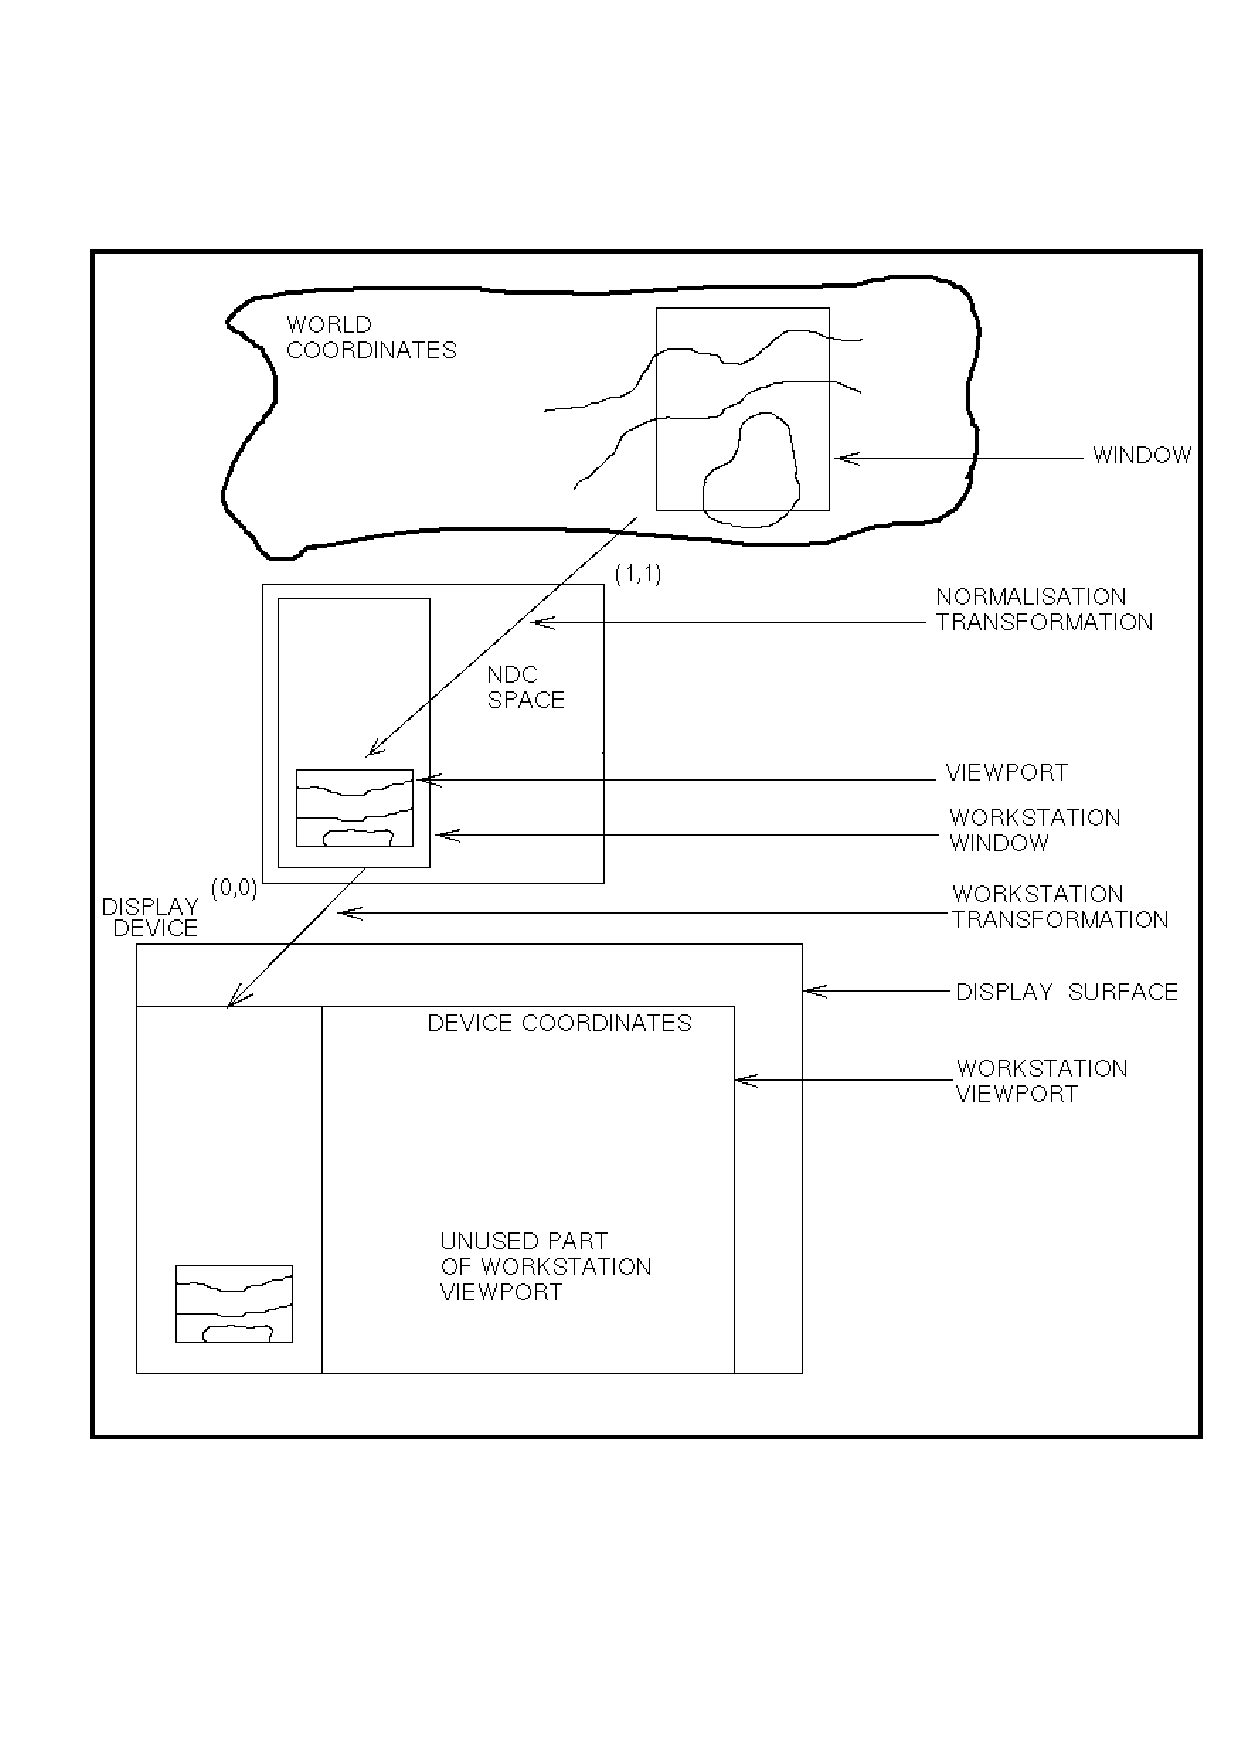
\includegraphics[scale=.8]{sun85_diag1}
%   \vspace{190mm}
   \caption{GKS Coordinate Systems}
\end{figure}

The {\bf workstation} is the complete
graphics station,
consisting of at least a display device and perhaps some input
devices as well.  An example of a workstation is a VDU with keyboard
and joystick;  the VDU is the display device in this case.  The
region of a display device on which images can be displayed
is called the {\bf display surface};  for
the example of the VDU the display surface is the addressable
area of the screen.

Moving now to the other end of the chain,
{\bf world coordinates} are those in which the user (i.e.\ the
programmer) wishes to work.  The units may be natural
for the information being plotted (counts versus \AA ngstroms
for example)
but equally often will simply be convenient units
for planning the picture.  (Note that the world coordinate x and y
always increase from left to right and from bottom to top;  this is a
fundamental property of GKS.)

The window is mapped onto the display surface by means of
a sequence of two independently
controllable transformations.  Each of the
two transformations proceeds from a `window'
to a `viewport'.

The first transformation, called the
{\bf normalisation transformation}, starts with the user's region
of interest in world coordinates which is called simply
the {\bf window}.  This maps onto an intermediate
system, called {\bf normalised device coordinates} (NDC);  the
NDC space consists
of a square region whose bottom left
and top right corners are respectively (0,0) and (1,1).  The
region within NDC space onto which the world coordinate
window maps is called the {\bf viewport}.

The second transformation is called the {\bf workstation
transformation}.  For each workstation, there
is a region in NDC space called the {\bf workstation
window}, and this maps onto part or
all of a region of the
display surface called the {\bf workstation viewport}.

The NDC space is an idealised model of the different
plotting devices;  in particular, the things plotted
in NDC space appear on the various devices without
change of shape---a circle in NDC space will appear
circular on all display devices, for example.  Because of this
conservation of aspect ratio, the workstation window
may not map onto the whole of the workstation
viewport, although this will commonly
be contrived.

The normalisation transformation allows
the window to be positioned
on the display surface without needing to refer to any
device units, and the workstation transformation
allows different workstations
to be treated separately.

Each workstation has its own workstation viewport and window and there can
be many window (world coordinates) to viewport (NDC)
transformations in existence,
the one used to transform output coordinates being selected by GSELNT.

\subsection* {Buffering}

Polylines and text strings are buffered within SGS and so at any time there
may be lines and text which have been `plotted' by SGS calls but have not yet
been passed to GKS (let alone output to the workstation).
Therefore any GKS calls should normally be preceded by a call to
\htmlref{SGS\_FLUSH}{SGS_FLUSH} to
ensure that all graphics activities are presented to GKS  in the correct order.

\subsection* {Transformations}

SGS only sets normalization transformation number 1.
Selecting a new zone is the only SGS activity that selects this to be the
current transformation.
Transformation 1 is used by
\htmlref{SGS\_SETCU}{SGS_SETCU} when it sets the locator position.

\htmlref{SGS\_SELZ}{SGS_SELZ}
 also sets the input priority of transformation 1 to be greater than
that of transformation 0 and the locator input routines expect transformation
1 to have the highest priority of all transformations.

\subsection* {Aspect source flags}

\htmlref{SGS\_OPEN}{SGS_OPEN} and \htmlref{SGS\_INIT}{SGS_INIT}
set the following aspect source flags:
\begin{description}
\item[\mbox{}]\mbox{}
\begin{description}
\item [POLYLINE] --- bundled
\item [POLYMARKER] --- individual
\item [TEXT] --- individual
\end{description}
\end{description}
SGS assumes these settings when it manipulates the polyline, marker and text
attributes.

\subsubsection* {Polylines}

Setting the SGS pen number simply sets the polyline index.
If the ASF for any attribute has been changed to individual then that attribute
will be unaffected by changing the SGS pen.
Pen numbers greater than 4 may be used provided that the corresponding polyline
index has been defined (either explicitly or by default).
If any polyline indices (or any other primitive index) are set explicitly then
this must be done before any drawing takes place, otherwise GKS will consider
that the picture needs to be regenerated.
When this happens, any drawing done outside a segment will be lost.
Since Close Workstation forces regeneration if it is required, the net effect is
for the workstation to be cleared when it is closed!

\subsubsection* {Markers}

When the SGS pen number is changed, the colour index of the new pen on the
current workstation is inquired and the polymarker colour index set to the same
value.
This results in markers being plotted in the same colour as lines {\em on the
current workstation}\/ but not necessarily on any other workstations that may be
active.
Activating a new workstation by selecting a new SGS zone modifies the colour
index to match the polylines on the new workstation.
If either the polyline colour index ASF has been set to individual or the
polymarker colour index ASF has been set to bundled, this mechanism will fail.

The SGS marker routines set the current marker type.
If the marker type ASF has been set to bundled, the marker type argument will
have no effect.

\subsubsection* {Text}

Text colour works in exactly the same way as marker colour and the same remarks
apply.
If any other text ASF is set to bundled, setting the corresponding SGS text
attribute will have no effect.

\section {SUBROUTINE SPECIFICATIONS}\label{app-subroutines}

\begin{latexonly}
The parameter descriptions have the following format:

\begin{tabular}{lll}
\em par&type&description
\end{tabular}

The `type' specifications use the following codes with the meanings shown:
\[\begin{tabular}{ll@{\hspace{1cm}}ll@{\hspace{1cm}}ll}
C&CHARACTER$\ast$($\ast$)&I&INTEGER&R&REAL\\
Cn&CHARACTER$\ast$n&L&LOGICAL
\end{tabular}\]
\end{latexonly}

\rthead{SGS\_APOLY}{Append new line to polyline}
\begin{description}
\item [ACTION:]
Adds a new line, whose end-point is ({\em x,y}), to an existing buffered
polyline.
It is possible that a partial polyline will be output automatically because of
finite buffer space (which however will be large).
SGS will, in this case, record that the polyline has to be continued but the
join might not be perfect in the case of dotted and dashed line-styles.
\item [CALL:]
{\tt SGS\_APOLY(x,y)}
\item [INPUT PARAMETERS:]
\begin{params}
\rparams{x,y}{R}{The end point of the line.}
\end{params}
\item [GKS EFFECT:]
If the current polyline buffer becomes full, then the polyline so far is sent to
GKS.
The specified point is added to the polyline buffer.
\end{description}
\goodbreak

\rthead{SGS\_ARC}{Draw arc of a circle}
\begin{description}
\item [ACTION:]
Draws an arc of a circle, centre ({\em x,y}), radius {\em r}, starting at
angle {\em theta1}\/ and finishing at angle {\em theta2}\/ in an anti-clockwise
direction.
\item [CALL:]
{\tt SGS\_ARC(x,y,r,theta1,theta2)}
\item [INPUT PARAMETERS:]
\begin{params}
\rparams{x,y}{R}{Centre of complete circle in world coordinates.}
\rparams{r}{R}{Radius of complete circle in world coordinates.}
\rparams{theta1,theta2}{R}{Start and finish angle of the arc in radians.
The angle increases anti-clockwise and 0 is at (x+r,y).}
\end{params}
\item [GKS EFFECT:]
Starts a new polyline (equivalent of SGS\_BPOLY).
Adds lines to the polyline, approximating the arc.
Finally, the polyline is sent to GKS.
The line length is chosen to correspond to the addressability of the finest
active workstation (inquiry is made of GKS to determine this).
\end{description}
\goodbreak

\rthead{SGS\_ATEXT}{Append a field to the text buffer}
\begin{description}
\item [ACTION:]
Appends to the SGS buffered text the entire specified CHARACTER expression (all
spaces included).
If the buffer would overflow, excess characters are lost.
\item [CALL:]
{\tt SGS\_ATEXT(string)}
\item [INPUT PARAMETERS:]
\begin{params}
\rparams{string}{C}{Text string to be appended entirely.}
\end{params}
\item [GKS EFFECT:]
None.
\end{description}
\goodbreak

\rthead{SGS\_ATXB}{Append to text with blanks}
\begin{description}
\item [ACTION:]
Appends to the SGS buffered text {\em nspace}\/ spaces followed by the specified
CHARACTER expression with all its leading spaces removed.
If the buffer would overflow, excess characters are lost.
\item [CALL:]
{\tt SGS\_ATXB(string,nspace)}
\item [INPUT PARAMETERS:]
\begin{params}
\rparams{string}{C}{Text string to be appended.}
\rparams{nspace}{I}{The exact number of spaces that are to be put in front of the
first non-space character appended to the buffer.}
\end{params}
\item [GKS EFFECT:]
None.
\end{description}
\goodbreak

\rthead{SGS\_ATXI}{Append to text an integer}
\begin{description}
\item [ACTION:]
Converts an integer to a character string, which is then placed in a field,
using {\em nfi}\/ as an indication of field width.
Appends the resulting field to the SGS buffered string.
\item [CALL:]
{\tt SGS\_ATXI(i,nfi)}
\item [INPUT PARAMETERS:]
\begin{params}
\rparams{i}{I}{Integer to be converted to characters.}
\rparams{nfi}{I}{Indicates what is to be done with the integer.}
\end{params}
\item [GKS EFFECT:]
None.
\item [NOTES:]
If $\mathit{nfi}\geq 0$, {\it nfi} spaces are appended to the SGS buffered
string, followed by the characters representing the number.
If $\mathit{nfi}<0$, the characters representing the number are put
right-justified into a field which is $-\mathit{nfi}$ characters wide.
If the field width is not sufficient, leading characters are lost.
\end{description}
\goodbreak

\rthead{SGS\_ATXL}{Append to text left justified}
\begin{description}
\item [ACTION:]
Appends to the SGS buffered text the specified CHARACTER expression with
trailing spaces removed.
If the buffer would overflow, excess characters are lost.
\item [CALL:]
{\tt SGS\_ATXL(string)}
\item [INPUT PARAMETERS:]
\begin{params}
\rparams{\em string}{C}{Text string to be appended.}
\end{params}
\item [GKS EFFECT:]
None.
\end{description}
\goodbreak

\rthead{SGS\_ATXR}{Append to text a real number}
\begin{description}
\item [ACTION:]
Converts a real number to a character string, using {\em ndp}\/ to determine the
number of decimal spaces.
Places the string in a field, using {\em nfi}\/ as an indication of field width.
Appends the field to the SGS buffered string.
\item [CALL:]
{\tt SGS\_ATXR(r,nfi,ndp)}
\item [INPUT PARAMETERS:]
\begin{params}
\rparams{r}{R}{Real number to be converted to characters.}
\rparams{nfi}{I}{Similarly to routine ATXI, this parameter indicates how the
converted real number is to be put in the field.}
\rparams{ndp}{I}{Indicates the number of digits after the decimal point.}
\end{params}
\item [GKS EFFECT:]
None.
\item [NOTES:]
If $\mathit{ndp}>0$, then {\it ndp}\/ digits are included.
If $\mathit{ndp}<0$, then only the integer part appears.
If $\mathit{ndp}=0$, then only the integer part and the decimal point appears.
\end{description}
\goodbreak

\rthead{SGS\_BOX}{Draw a box\hfill {\bf SGS\_BOX}}
\begin{description}
\item [ACTION:]
Draws a rectangular box with sides parallel to the axes.
\item [CALL:]
{\tt SGS\_BOX(x1,x2,y1,y2)}
\item [INPUT PARAMETERS:]
\begin{params}
\rparams{x1,x2,y1,y2}{R}{Extent of box in world coordinates.}
\end{params}
\item [GKS EFFECT:]
A polyline is drawn (via \htmlref{SGS\_BPOLY}{SGS_BPOLY} and
\htmlref{SGS\_APOLY}{SGS_APOLY}).
\end{description}
\goodbreak

\rthead{SGS\_BPOLY}{Begin polyline}
\begin{description}
\item [ACTION:]
Indicates that a new chain of lines (could be only one line) is to begin at the
specified point.
Further end points are added by \htmlref{SGS\_APOLY}{SGS_APOLY}.
Any existing buffered polyline is output first.
\item [CALL:]
{\tt SGS\_BPOLY(x,y)}
\item [INPUT PARAMETERS:]
\begin{params}
\rparams{\em x,y}{R}{Starting coordinates for polyline.}
\end{params}
\item [GKS EFFECT:]
Any existing buffered polyline is output first by calling the GKS polyline
routine.
Then the starting position of the new polyline is saved.
\end{description}
\goodbreak

\rthead{SGS\_BTEXT}{Begin a new text string}
\begin{description}
\item [ACTION:]
Flushes the SGS buffered string if one exists, and sets up a new one with zero
characters.
The reference point is recorded.
\item [CALL:]
{\tt SGS\_BTEXT(x,y)}
\item [INPUT PARAMETERS:]
\begin{params}
\rparams{x,y}{R}{Reference point in world coordinates.
This is used when the buffer is flushed.}
\end{params}
\item [GKS EFFECT:]
The current text string (if it exists) is sent to GKS.
\end{description}
\goodbreak

\rthead{SGS\_BZNDC}{Set a base zone extent in NDC}
\begin{description}
\item [ACTION:]
Sets the extent in NDC of a base zone.
\item [CALL:]
{\tt SGS\_BZNDC(x1,x2,y1,y2,pos,istat)}
\item [INPUT PARAMETERS:]
\begin{params}
\rparams{x1,x2,y1,y2}{R}{Extent of zone in normalised device coordinates.}
\rparams{pos}{C2}{Determines the positioning of the zone on the display surface.
The first character is `B', `C' or `T' (standing for bottom, centre and top), and
the second is `L', `C' or `R' (standing for left, centre and right).}
\end{params}
\item [OUTPUT PARAMETERS:]
\begin{params}
\rparams{istat}{I}{Status.}
\end{params}
\item [GKS EFFECT:]
The viewport and workstation window are set to the requested NDC values, and the
workstation viewport set to the largest rectangle of the same aspect ratio that
will fit on the display surface, and positioned as specified.
\end{description}
\goodbreak

\rthead{SGS\_CIRCL}{Draw circle}
\begin{description}
\item [ACTION:]
Draws a complete circle, centre ({\em x,y}), radius {\em r}.
\item [CALL:]
{\tt SGS\_CIRCL(x,y,r)}
\item [INPUT PARAMETERS:]
\begin{params}
\rparams{x,y}{R}{Centre of circle in world coordinates.}
\rparams{r}{R}{Radius of circle in world coordinates.}
\end{params}
\item [GKS EFFECT:]
Similar to ARC routine except that complete circle is drawn.
\end{description}
\goodbreak

\rthead{SGS\_CLOSE}{Close graphics}
\begin{description}
\item [ACTION:]
Puts out the SGS text and polyline buffers.
Closes GKS.
\item [CALL:]
{\tt SGS\_CLOSE}
\item [GKS EFFECT:]
All pending output dispatched (via \htmlref{SGS\_FLUSH}{SGS_FLUSH}).
All active workstations are deactivated.
All open workstations are closed.
GKS is closed.
\end{description}
\goodbreak

\rthead{SGS\_CLRBL}{Clear block}
\begin{description}
\item [ACTION:]
Clears specified area of screen if this can be done without affecting the rest
of the display surface.
\item [CALL:]
{\tt SGS\_CLRBL(x1,x2,y1,y2)}
\item [INPUT PARAMETERS:]
\begin{params}
\rparams{x1,x2,y1,y2}{R}{Extent of area in world coordinates.}
\end{params}
\item [GKS EFFECT:]
The specified area is cleared.
The technique used depends on the workstation type.
\end{description}
\goodbreak

\rthead{SGS\_CLRFG}{Set clear screen flag}
\begin{description}
\item [ACTION:]
Sets or clears the `suppress clear screen flag on open workstation' according
to the {\em iflag}\/ argument.
N.B.\ This function is specific to RAL GKS and is not implemented on all
workstations.
\item [CALL:]
{\tt SGS\_CLRFG(iflag)}
\item [INPUT PARAMETERS:]
\begin{params}
\rparams{iflag}{I}{1 disables screen clearing on open; 0 restores the normal
GKS behaviour.}
\end{params}
\item [GKS EFFECT:]
GESC is called with escape number 1000.
\end{description}
\goodbreak

\rthead{SGS\_CLRZ}{Clear zone}
\begin{description}
\item [ACTION:]
Clears the current zone.
The entire display surface may be cleared on some devices.
\item [CALL:]
{\tt SGS\_CLRZ}
\item [GKS EFFECT:]
If the device is capable of selective erasure
\htmlref{SGS\_CLRBL}{SGS_CLRBL} is called, otherwise
the entire display surface is cleared.
\end{description}
\goodbreak

\rthead{SGS\_CLSWK}{Close workstation}
\begin{description}
\item [ACTION:]
Puts out the SGS text and polyline buffers.
If there are no other base zones on the workstation, releases all zones
associated with the workstation, deactivates and closes the workstation.
Otherwise, the specified zone is released.
\item [CALL:]
{\tt SGS\_CLSWK(izonid,istat)}
\item [INPUT PARAMETERS:]
\begin{params}
\rparams{izonid}{I}{Zone identifier for a base zone on this workstation.}
\end{params}
\item [OUTPUT PARAMETERS:]
\begin{params}
\rparams{istat}{I}{If workstation is closed OK, then this value is zero.}
\end{params}
\item [GKS EFFECT:]
All pending output dispatched (via \htmlref{SGS\_FLUSH}{SGS_FLUSH}).
The appropriate workstation may be deactivated and closed.
\end{description}
\goodbreak

\rthead{SGS\_CUVIS}{Set cursor visibility}
\begin{description}
\item [ACTION:]
Sets the visibility of the cursor on the current SGS workstation.
\item [CALL:]
{\tt SGS\_CUVIS(vis)}
\item [INPUT PARAMETERS:]
\begin{params}
\rparams{vis}{L}{The visibility of the cursor.}
\end{params}
\item [GKS EFFECT:]
The echo switch for locator device 1 is set.
\end{description}
\goodbreak

\rthead{SGS\_DEFCH}{Define valid choice keys}
\begin{description}
\item [ACTION:]
Defines the valid keys for choice input from the command terminal
keyboard (SGS choice device type 0).
\item [CALL:]
{\tt SGS\_DEFCH(chostr)}
\item [INPUT PARAMETERS:]
\begin{params}
\rparams{chostr}{C}{A character expression of up to 49 characters which defines
the keys that are valid for choice input. The order of the characters
determines the number returned when a key is pressed. The first key in the
string will return 1, the second 2, etc. If a key which has not been defined
is pressed, a 0 is returned.}
\end{params}
\item [GKS EFFECT:]
None
\end{description}
\goodbreak

\rthead{SGS\_DISCU}{Disable sample cursor}
\begin{description}
\item [ACTION:]
Disables sample mode for the cursor.
\item [CALL:]
{\tt SGS\_DISCU}
\item [GKS EFFECT:]
The mode of locator device 1 on the current SGS workstation is set to REQUEST.
\end{description}
\goodbreak

\rthead{SGS\_ENSCU}{Enable sample cursor}
\begin{description}
\item [ACTION:]
Enables sample mode for the cursor.
\item [CALL:]
{\tt SGS\_ENSCU}
\item [GKS EFFECT:]
The mode of locator device 1 on the current SGS workstation is set to SAMPLE.
\end{description}
\goodbreak

\rthead{SGS\_FLUSH}{Flush buffers}
\begin{description}
\item [ACTION:]
Flushes all buffers.
\item [CALL:]
{\tt SGS\_FLUSH}
\item [GKS EFFECT:]
Flushes the SGS text and line buffers before calling GUWK for all active
workstations to flush the GKS buffers.
\end{description}
\goodbreak

\rthead{SGS\_ICUAV}{Inquire cursor availability}
\begin{description}
\item [ACTION:]
Sets {\em avail}\/ to .TRUE. if a cursor is available on the current SGS device,
and to .FALSE. otherwise.
\item [CALL:]
{\tt SGS\_ICUAV(avail)}
\item [OUTPUT PARAMETERS:]
\begin{params}
\rparams{avail}{L}{.TRUE. or .FALSE., depending on the availability of a
cursor.}
\end{params}
\item [GKS EFFECT:]
Inquires only.
\end{description}
\goodbreak

\rthead{SGS\_ICURW}{Inquire current workstation}
\begin{description}
\item [ACTION:]
Returns workstation ID for current zone.
\item [CALL:]
{\tt SGS\_ICURW(iwkid)}
\item [OUTPUT PARAMETERS:]
\begin{params}
\rparams{iwkid}{I}{The workstation ID for the SGS zone last selected.}
\end{params}
\item [GKS EFFECT:]
None.
\end{description}
\goodbreak

\rthead{SGS\_ICURZ}{Inquire current zone}
\begin{description}
\item [ACTION:]
Returns ID of current SGS zone.
\item [CALL:]
{\tt SGS\_ICURZ(izonid)}
\item [OUTPUT PARAMETERS:]
\begin{params}
\rparams{izonid}{I}{Identifier of last selected SGS zone.}
\end{params}
\item [GKS EFFECT:]
None.
\end{description}
\goodbreak

\rthead{SGS\_IDUN}{Inquire device units}
\begin{description}
\item [ACTION:]
Obtains the length of device units in each of x and y for the current SGS zone.
\item [CALL:]
{\tt SGS\_IDUN(dxw,dyw)}
\item [OUTPUT PARAMETERS:]
\begin{params}
\rparams{dxw,dyw}{R}{Size of a raster unit in world coordinates in each of the
x and y directions.}
\end{params}
\item [GKS EFFECT:]
Inquires only.
\end{description}
\goodbreak

\rthead{SGS\_INCHO}{Inquire number of choices}
\begin{description}
\item [ACTION:]
Inquires the number of choices available on the currently selected workstation.
\item [CALL:]
{\tt SGS\_INCHO(nchoic,n)}
\item [INPUT PARAMETERS:]
\begin{params}
\rparams{nchoic}{I}{The SGS choice device number:
1 or greater is a GKS choice device, 0 is the command terminal.}
\end{params}
\item [OUTPUT PARAMETERS:]
\begin{params}
\rparams{n}{I}{The number of choices available on the selected device.
If no such device exists, zero will be returned.}
\end{params}
\item [GKS EFFECT:]
Inquires only.
\end{description}
\goodbreak

\rthead{SGS\_INIT}{Initialize SGS}
\begin{description}
\item [ACTION:]
Initializes SGS and (if necessary) opens GKS.
\item [CALL:]
{\tt SGS\_INIT(lun,istat)}
\item [INPUT PARAMETERS:]
\begin{params}
\rparams{lun}{I}{Logical unit number for error messages.}
\end{params}
\item [OUTPUT PARAMETERS:]
\begin{params}
\rparams{istat}{I}{Status; set to 0 if SGS is successfully initialized.}
\end{params}
\item [GKS EFFECT:]
If GKS is not already open GOPKS is called with the specified logical unit
number as the error channel.
\end{description}
\goodbreak

\rthead{SGS\_IPEN}{Inquire pen number}
\begin{description}
\item [ACTION:]
Returns current SGS pen number.
\item [CALL:]
{\tt SGS\_IPEN(npen)}
\item [OUTPUT PARAMETERS:]
\begin{params}
\rparams{npen}{I}{The current SGS pen number as presented via SGS\_SPEN.}
\end{params}
\item [GKS EFFECT:]
None.
\end{description}
\goodbreak

\rthead{SGS\_IPLXY}{Inquire polyline x and y}
\begin{description}
\item [ACTION:]
Returns the coordinates of the last line added to the polyline buffer, if there
is one.
\item [CALL:]
{\tt SGS\_IPLXY(x,y)}
\item [OUTPUT PARAMETERS:]
\begin{params}
\rparams{x,y}{R}{{\em x}\/ and {\em y}\/ of the last line added to the polyline
buffer, if there is such a line. If not, {\em x}\/ and {\em y}\/ are unchanged.}
\end{params}
\item [GKS EFFECT:]
None.
\end{description}
\goodbreak

\rthead{SGS\_ISLER}{Inquire selective erase capability}
\begin{description}
\item [ACTION:]
Sets {\em blker}\/ to .TRUE. if the current workstation is capable of clearing
selected areas of the display; if not it is set to .FALSE..
\item [CALL:]
{\tt SGS\_ISLER(blker)}
\item [OUTPUT PARAMETERS:]
\begin{params}
\rparams{blker}{L}{.TRUE. or .FALSE. depending on whether device has
selective erase capability.}
\end{params}
\item [GKS EFFECT:]
None.
\end{description}
\goodbreak

\rthead{SGS\_ITXA}{Inquire text attributes}
\begin{description}
\item [ACTION:]
Returns the values of all the SGS text attributes.
\item [CALL:]
{\tt SGS\_ITXA(nf,npr,ht,ar,xu,yu,sp,txj)}
\item [OUTPUT PARAMETERS:]
\begin{params}
\rparams{nf,npr}{I}{Font number and text precision.}
\rparams{ht,ar}{R}{Character height, aspect ratio.}
\rparams{xu,yu}{R}{Text orientation direction cosines.}
\rparams{sp}{R}{Text spacing.}
\rparams{txj}{C2}{Text alignment coding.}
\end{params}
\item [GKS EFFECT:]
None.
\end{description}
\goodbreak

\rthead{SGS\_ITXB}{Inquire text buffer}
\begin{description}
\item [ACTION:]
Returns state of SGS buffered string.
\item [CALL:]
{\tt SGS\_ITXB(x,y,n,dx,dy)}
\item [OUTPUT PARAMETERS:]
\begin{params}
\rparams{x,y}{R}{Reference position of SGS buffered string.}
\rparams{n}{I}{Number of characters in buffered string.}
\rparams{dx,dy}{R}{The extent of the current buffered string (expressed as a
displacement from its starting point).}
\end{params}
\item [GKS EFFECT:]
Inquiry is made of GKS to determine the concatenation point, from
which {\em x}\/ and {\em y}\/ are subtracted to give the SGS extent.
\end{description}
\goodbreak

\rthead{SGS\_IZONE}{Inquire zone attributes}
\begin{description}
\item [ACTION:]
Returns bounds and size of current SGS zone.
\item [CALL:]
{\tt SGS\_IZONE(x1,x2,y1,y2,xm,ym)}
\item [OUTPUT PARAMETERS:]
\begin{params}
\rparams{x1,x2,y1,y2}{R}{Bounds of current zone.}
\rparams{xm,ym}{R}{Size of zone in metres.}
\end{params}
\item [GKS EFFECT:]
The workstation transformation for the workstation of the current SGS zone is
inquired via GQWKT.
\end{description}
\goodbreak

\rthead{SGS\_LINE}{Begin polyline with single line}
\begin{description}
\item [ACTION:]
Starts a new polyline with the specified line.
If subsequent lines are added, the first 2 points will be ({\em x1,y1}) and
{\em (x2,y2)}.
\item [CALL:]
{\tt SGS\_LINE(x1,y1,x2,y2)}
\item [INPUT PARAMETERS:]
\begin{params}
\rparams{x1,y1}{R}{Coordinates of the first point on the polyline.}
\rparams{x2,y2}{R}{End point of the line.}
\end{params}
\item [GKS EFFECT:]
Effect is same as {\tt CALL SGS\_BPOLY({\em x1},{\em y1})} then {\tt CALL
SGS\_APOLY({\em x2},{\em y2})}.
\end{description}
\goodbreak

\rthead{SGS\_MARK}{Draw marker}
\begin{description}
\item [ACTION:]
Draws a single marker, centred on the given position ({\em x,y}).
\item [CALL:]
{\tt SGS\_MARK(x,y,mtype)}
\item [INPUT PARAMETERS:]
\begin{params}
\rparams{x,y}{R}{Coordinates of the marker.}
\rparams{mtype}{I}{Marker type.}
\end{params}
\item [GKS EFFECT:]
The current marker type is set to {\em mtype}\/ and a marker is output using the
GKS polymarker routine GPM.
No SGS buffers are affected.
\item [NOTES:]
The correspondence between marker types and marker shapes is shown in
\hyperref{this section}{section~}{}{sec-markers}.
\end{description}
\goodbreak

\rthead{SGS\_MARKL}{Draw marker at end of polyline}
\begin{description}
\item [ACTION:]
If there is an SGS buffered polyline, it is output, a marker is output at its
end position and a new buffered polyline is begun.
\item [CALL:]
{\tt SGS\_MARKL(mtype)}
\item [INPUT PARAMETERS:]
\begin{params}
\rparams{mtype}{I}{Marker type.}
\end{params}
\item [GKS EFFECT:]
Current buffered polyline is output via GKS; the current marker type is set to
{\em mtype}\/ and a marker is output at the end position using the GKS polymarker
routine GPM; a new SGS buffered polyline is begun.
\item [NOTES:]
Same as SGS\_MARK.
\end{description}
\goodbreak

\rthead{SGS\_OPEN}{Open graphics}
\begin{description}
\item [ACTION:]
Performs all GKS calls necessary to get the specified workstation open and
active.
Also sets defaults for various attributes and should therefore be used if
other SGS routines are called.
It is intended to be used at the beginning of graphics.
\item [CALL:]
{\tt SGS\_OPEN(wkstn,izonid,istat)}
\item [INPUT PARAMETERS:]
\begin{params}
\rparams{wkstn}{C}{Workstation name: a character string which translates
ultimately into GKS workstation sequence number and connection identifier.
See \xref{SUN/57}{sun57}{}
for full details of formats supported; simplest is the two numbers
as decimals separated by a comma.}
\end{params}
\item [OUTPUT PARAMETERS:]
\begin{params}
\rparams{izonid}{I}{Zone identifier for the base SGS zone on this workstation;
allocated by SGS.}
\rparams{istat}{I}{If workstation is opened OK, then this value is zero.}
\end{params}
\item [GKS EFFECT:]
If GKS is already open it is left open; otherwise it is opened with logical
unit 22 as the error channel.
The specified workstation is opened and activated.
Maximum deferral is requested.
An SGS base zone filling the display surface is set up.
The polyline aspect source flags are set to bundled and the marker and text
aspect source flags set to individual.
\end{description}
\goodbreak

\rthead{SGS\_OPNWK}{Open workstation}
\begin{description}
\item [ACTION:]
Opens an additional workstation, and sets up the base SGS zone, which is then
selected.
\item [CALL:]
{\tt SGS\_OPNWK(wkstn,izonid,istat)}
\item [INPUT PARAMETERS:]
\begin{params}
\rparams{wkstn}{C}{Workstation type/connection identifier pair (see SGS\_OPEN).}
\end{params}
\item [OUTPUT PARAMETERS:]
\begin{params}
\rparams{izonid}{I}{Zone identifier---number allocated by SGS.}
\rparams{istat}{I}{If workstation is opened OK, this value is 0.}
\end{params}
\item [GKS EFFECT:]
Unless already opened by SGS the specified workstation is opened; the
workstation viewport is set to cover the full display surface.
A base zone is set up and selected via \htmlref{SGS\_SELZ}{SGS_SELZ}.
\end{description}
\goodbreak

\rthead{SGS\_OPOLY}{Output buffered polyline}
\begin{description}
\item [ACTION:]
Outputs buffered polyline.
SGS\_OPOLY is automatically invoked, at appropriate times, by other routines and
only rarely requires calling directly.
\item [CALL:]
{\tt SGS\_OPOLY}
\item [GKS EFFECT:]
The buffered polyline is sent to GKS.
\end{description}
\goodbreak

\rthead{SGS\_OTEXT}{Output buffered text}
\begin{description}
\item [ACTION:]
Outputs existing SGS buffered text.
The point stored by \htmlref{SGS\_BTEXT}{SGS_BTEXT}
is used as the reference point.
Current text attributes are used, including the SGS text alignment.
SGS\_OTEXT is automatically invoked, at appropriate times, by other routines and
rarely needs to be called directly.
\item [CALL:]
{\tt SGS\_OTEXT}
\item [GKS EFFECT:]
The current text string is sent to GKS.
\end{description}
\goodbreak

\rthead{SGS\_RELZ}{Release zone}
\begin{description}
\item [ACTION:]
Offers the specified SGS zone for release.
\item [CALL:]
{\tt SGS\_RELZ(izonid)}
\item [INPUT PARAMETERS:]
\begin{params}
\rparams{izonid}{I}{The identifier for the SGS zone which the program no longer
requires.}
\end{params}
\item [GKS EFFECT:]
None.
\end{description}
\goodbreak

\rthead{SGS\_REQCH}{Request choice}
\begin{description}
\item [ACTION:]
Waits for the user to press a key on the current SGS choice device
and returns the number of the key selected.
When choice device 0 is being used, the number is the position in the define
keys string passed to \htmlref{SGS\_DEFCH}{SGS_DEFCH}.
If the key is not included in the string, 0 is returned.
\item [CALL:]
{\tt SGS\_REQCH(n)}
\item [OUTPUT PARAMETERS:]
\begin{params}
\rparams{n}{I}{The number of the key pressed.}
\end{params}
\item [GKS EFFECT:]
All buffered output is plotted and for device 1 GKS request choice is called.
\end{description}
\goodbreak

\rthead{SGS\_REQCU}{Request cursor position}
\begin{description}
\item [ACTION:]
Waits for the user to press a key on the current SGS choice device
and then returns the position of the cursor and the number of the choice key.
\item [CALL:]
{\tt SGS\_REQCU(x,y,n)}
\item [OUTPUT PARAMETERS:]
\begin{params}
\rparams{x,y}{R}{The cursor position in world coordinates.}
\rparams{n}{I}{The number of the key pressed.}
\end{params}
\item [GKS EFFECT:]
GKS request locator is called.
If the current choice device is not 0, GKS request choice is called.
\end{description}
\goodbreak

\rthead{SGS\_SAMCU}{Sample cursor}
\begin{description}
\item [ACTION:]
Returns the cursor position without waiting for the user to press any key.
\item [CALL:]
{\tt SGS\_SAMCU(x,y)}
\item [OUTPUT PARAMETERS:]
\begin{params}
\rparams{x,y}{R}{The cursor position in world coordinates.}
\end{params}
\item [GKS EFFECT:]
All output buffers are plotted and locator device 1 is sampled on the
current SGS workstation.
\end{description}
\goodbreak

\rthead{SGS\_SARTX}{Set aspect ratio of text}
\begin{description}
\item [ACTION:]
Sets aspect ratio (width/height) of text.
A usual figure is between 1/1.3 and 1/1.5; the default is 2/3.
\item [CALL:]
{\tt SGS\_SARTX(ar)}
\item [INPUT PARAMETERS:]
\begin{params}
\rparams{ar}{R}{Aspect ratio.}
\end{params}
\item [GKS EFFECT:]
Outputs any SGS buffered text, sets SGS aspect ratio and resets all GKS text
attributes to follow current SGS settings.
\end{description}
\goodbreak

\rthead{SGS\_SELCH}{Select choice device}
\begin{description}
\item [ACTION:]
Selects the current SGS choice device.
\item [CALL:]
{\tt SGS\_SELCH(nchdev)}
\item [INPUT PARAMETERS:]
\begin{params}
\rparams{nchdev}{I}{The SGS choice device to be used for subsequent input:
1 or greater is a GKS choice device number, 0 is the command terminal.}
\end{params}
\item [GKS EFFECT:]
None.
\end{description}
\goodbreak

\rthead{SGS\_SELZ}{Select zone}
\begin{description}
\item [ACTION:]
Selects the nominated SGS zone.
\item [CALL:]
{\tt SGS\_SELZ(izonid,istat)}
\item [INPUT PARAMETERS:]
\begin{params}
\rparams{izonid}{I}{The zone identifier supplied by SGS when the zone was set
up.}
\rparams{istat}{I}{If the zone is selected successfully, then this value is 0.}
\end{params}
\item [GKS EFFECT:]
If the new zone is on a different workstation from the current zone, the current
workstation is deactivated and the new one activated and the marker and text
indices are set to those of the current SGS pen.
Normalization transformation number 1 is selected and a new window/viewport is
set up.
\end{description}
\goodbreak

\rthead{SGS\_SETCU}{Set cursor position}
\begin{description}
\item [ACTION:]
Sets the cursor to the specified position, provided that the hardware is capable
of this.
If the cursor is not visible, it will appear at the requested position when it
next becomes visible.
If the requested position is outside the workstation window, no action is taken.
\item [CALL:]
{\tt SGS\_SETCU(x,y)}
\item [INPUT PARAMETERS:]
\begin{params}
\rparams{x,y}{R}{The desired cursor position in world coordinates.}
\end{params}
\item [GKS EFFECT:]
Initialize Locator called with ({\em x,y}) as the new initial position and
transformation 1 as the initial transformation.
Other attributes are unchanged.
\end{description}
\goodbreak

\rthead{SGS\_SFONT}{Set font of text}
\begin{description}
\item [ACTION:]
Sets font number.
\item [CALL:]
{\tt SGS\_SFONT(nf)}
\item [INPUT PARAMETERS:]
\begin{params}
\rparams{nf}{I}{Font number.
The default is 1.
See the GKS user guide for details of other available fonts.}
\end{params}
\item [GKS EFFECT:]
Outputs any SGS buffered text, sets SGS font number, selects GKS font
and precision.
\end{description}
\goodbreak

\rthead{SGS\_SHTX}{Set height of text}
\begin{description}
\item [ACTION:]
Sets character height.
Default is 0.02.
\item [CALL:]
{\tt SGS\_SHTX(ht)}
\item [INPUT PARAMETERS:]
\begin{params}
\rparams{ht}{R}{Character height in world coordinates.}
\end{params}
\item [GKS EFFECT:]
Outputs any SGS buffered text, sets SGS character height and sets GKS text
attributes from the SGS settings.
\item [NOTES:]
If the coordinate system changes, then the displayed size will alter.
The program would then have to supply a new value to maintain the same display
size.
\end{description}
\goodbreak

\rthead{SGS\_SPEN}{Select pen}
\begin{description}
\item [ACTION:]
Selects SGS pen.
Any polyline or text string is flushed first.
The initial pen is number 1.
\item [CALL:]
{\tt SGS\_SPEN(npen)}
\item [INPUT PARAMETERS:]
\begin{params}
\rparams{npen}{I}{Required SGS pen number.}
\end{params}
\item [GKS EFFECT:]
The GKS pen number is set to the SGS pen number given.
All available workstations are assumed to support at least 4 predefined pens,
giving readily distinguishable lines.
The marker and text colour indices are set to the same value as for polylines on
the current SGS workstation.
\end{description}
\goodbreak

\rthead{SGS\_SPREC}{Set precision of text}
\begin{description}
\item [ACTION:]
Sets text precision.
This indicates the fidelity with which the text attributes are followed by GKS.
Precision 2 (the SGS default) is the most accurate and is normally achieved by
a software font.
\item [CALL:]
{\tt SGS\_SPREC(npr)}
\item [INPUT PARAMETERS:]
\begin{params}
\rparams{npr}{I}{Text precision.}
\end{params}
\item [GKS EFFECT:]
Outputs any SGS buffered text, sets SGS precision number, sets GKS font and
precision.
\end{description}
\goodbreak

\rthead{SGS\_SSPTX}{Set spacing of text}
\begin{description}
\item [ACTION:]
Sets text spacing.
Default is 0.0.
\item [CALL:]
{\tt SGS\_SSPTX(sp)}
\item [INPUT PARAMETERS:]
\begin{params}
\rparams{sp}{R}{Spacing between the end of one character and the start of the
next.}
\end{params}
\item [GKS EFFECT:]
Outputs any SGS buffered text.
Sets GKS text attributes from the SGS settings.
\item [NOTES:]
Spacing in SGS is expressed as a fraction of the nominal width of the character
box.
\end{description}
\goodbreak

\rthead{SGS\_STXJ}{Set text justification}
\begin{description}
\item [ACTION:]
Sets the alignment options that are subsequently used by SGS\_OTEXT
and by implicit and explicit flushes of the SGS text buffer.
\item [CALL:]
{\tt SGS\_STXJ(txj)}
\item [INPUT PARAMETERS:]
\begin{params}
\rparams{txj}{C2}{A 2 letter option string.}
\end{params}
\item [GKS EFFECT:]
Outputs SGS buffered text.
Sets GKS text attributes from SGS settings.
\item [NOTES:]
The 1st letter is the vertical alignment: B(OTTOM), C(ENTRE) or T(OP).
The 2nd is the horizontal alignment: L(EFT), C(ENTRE) or R(IGHT).
In either case, space implies no change.
The default is `BL'.
The alignment refers to where in the character string the nominated X,Y lies;
thus a code of `BL' would place the nominated X,Y at the bottom left of the
string.
The terms `top', `left' etc.\ refer to the character string as seen in its
conventional orientation, rather than as actually displayed.
\end{description}
\goodbreak

\rthead{SGS\_SUPTX}{Set up vector of text}
\begin{description}
\item [ACTION:]
Specifies character orientation in terms of a vector.
Default is (0.0,1.0).
\item [CALL:]
{\tt SGS\_SUPTX(xu,yu)}
\item [INPUT PARAMETERS:]
\begin{params}
\rparams{xu,yu}{R}{A vector specifying the up direction of subsequent text.}
\end{params}
\item [GKS EFFECT:]
Outputs any SGS buffered text.
Sets GKS text attributes from SGS settings.
\item [NOTES:]
The vector is the direction of the vertical axis of each character.
The standard orientation would be (0.0,1.0).
Only the direction of the vector, not its magnitude, is significant.
\end{description}
\goodbreak

\rthead{SGS\_SW}{Set window}
\begin{description}
\item [ACTION:]
Sets the bounds of plotting in world coordinates.
\item [CALL:]
{\tt SGS\_SW(x1,x2,y1,y2,istat)}
\item [INPUT PARAMETERS:]
\begin{params}
\rparams{x1,x2}{R}{Left and right bounds in X.}
\rparams{y1,y2}{R}{Bottom and top bounds in Y.}
\rparams{istat}{I}{Status.}
\end{params}
\item [GKS EFFECT:]
Sets the window bounds for normalization transformation number 1 according to
the parameters provided.
The {\it x1,x2} and {\it y1,y2} values are sorted so that $\mathit{x2}>
\mathit{x1}$ and $\mathit{y2}>\mathit{y1}$ before the GKS transformation is set up.
\end{description}
\goodbreak

\rthead{SGS\_TPZ}{Transform position to new zone}
\begin{description}
\item [ACTION:]
Translates a position in zone IZIN to its corresponding position in zone IZOUT.
\item [CALL:]
{\tt SGS\_TPZ(izin,xin,yin,izout,xout,yout,istat)}
\item [INPUT PARAMETERS:]
\begin{params}
\rparams{izin}{I}{ID of zone of input position.}
\rparams{xin,yin}{R}{Position to be transformed.}
\rparams{izout}{I}{ID of zone to which the position is to be transformed.}
\end{params}
\item [OUTPUT PARAMETERS:]
\begin{params}
\rparams{xout,yout}{R}{Output position.}
\rparams{istat}{I}{Status.}
\end{params}
\item [GKS EFFECT:]
None.
\end{description}
\goodbreak

\rthead{SGS\_TX}{Begin a new text string with a string}
\begin{description}
\item [ACTION:]
Starts a new SGS buffered text string with the specified text.
\item [CALL:]
{\tt SGS\_TX(x,y,string)}
\item [INPUT PARAMETERS:]
\begin{params}
\rparams{x,y}{R}{Reference point for new SGS buffered string.}
\rparams{string}{C}{Text string to be put into emptied text buffer.}
\end{params}
\item [GKS EFFECT:]
A new SGS buffered string is begun: equivalent to
\htmlref{SGS\_BTEXT}{SGS_BTEXT}(x,y); the
specified string is appended to it: equivalent to
\htmlref{SGS\_ATEXT}{SGS_ATEXT}(string)
\end{description}
\goodbreak

\rthead{SGS\_TXI}{Begin new text with integer}
\begin{description}
\item [ACTION:]
Starts a new SGS buffered text string with text derived from the specified
integer.
\item [CALL:]
{\tt SGS\_TXI(x,y,i,nfi)}
\item [INPUT PARAMETERS:]
\begin{params}
\rparams{x,y}{R}{Reference point of new SGS buffered string.}
\rparams{i}{I}{Integer to be converted to characters.}
\rparams{nfi}{I}{Indication of field width: similar to
\htmlref{SGS\_ATXI}{SGS_ATXT}.}
\end{params}
\item [GKS EFFECT:]
A new SGS buffered string is begun: equivalent to
\htmlref{SGS\_BPOLY}{SGS_BPOLY}(x,y).
The converted integer is appended to it: equivalent to
\htmlref{SGS\_ATXI}{SGS_ATXI}(i,nfi).
\end{description}
\goodbreak

\rthead{SGS\_TXR}{Begin new text with real}
\begin{description}
\item [ACTION:]
Starts a new SGS buffered string with text derived from the specified real
number.
\item [CALL:]
{\tt SGS\_TXR(x,t,r,nfi,ndp)}
\item [INPUT PARAMETERS:]
\begin{params}
\rparams{x,y}{R}{Reference point of new SGS buffered string.}
\rparams{r}{R}{Real number to be converted to characters.}
\rparams{nfi,ndp}{I}{Conversion parameters, similar to
\htmlref{SGS\_ATXR}{SGS_ATXR}.}
\end{params}
\item [GKS EFFECT:]
A new SGS buffered string is begun: equivalent to
\htmlref{SGS\_APOLY}{SGS_APOLY}(x,y).
The converted real number is appended: equivalent to
\htmlref{SGS\_ATXR}{SGS_ATXR}(r,nfi,ndp).
\end{description}
\goodbreak

\rthead{SGS\_WIDEN}{Translate SGS workstation name to GKS}
\begin{description}
\item [ACTION:]
Translates the SGS workstation name to its equivalent GKS workstation type
and connection identifier.
May be called before SGS\_OPEN.
\item [CALL:]
{\tt SGS\_WIDEN(wkstn,itype,iconid,istat)}
\item [INPUT PARAMETERS:]
\begin{params}
\rparams{wkstn}{C}{SGS workstation name.}
\end{params}
\item [OUTPUT PARAMETERS:]
\begin{params}
\rparams{itype}{I}{GKS workstation type.}
\rparams{iconid}{I}{GKS connection identifier.}
\rparams{istat}{I}{Status. Set to zero if translation was possible.}
\end{params}
\item [GKS EFFECT:]
None.
\end{description}
\goodbreak

\rthead{SGS\_WLIST}{List available workstations}
\begin{description}
\item [ACTION:]
Outputs a list of the SGS workstation names that have been defined on the
specified FORTRAN logical unit.
This routine may be called before \htmlref{SGS\_OPEN}{SGS_OPEN}.
\item [CALL:]
{\tt SGS\_WLIST(LUN)}
\item [INPUT PARAMETERS:]
\begin{params}
\rparams{lun}{I}{FORTRAN logical unit number.}
\end{params}
\item [GKS EFFECT:]
As for SGS\_WNAME
\end{description}
\goodbreak

\rthead{SGS\_WNAME}{Generate list of workstation names}
\begin{description}
\item [ACTION:]
Passes a list of the SGS workstation names that have been defined to the
specified action routine.
May be called before SGS\_OPEN.
\item [CALL:]
{\tt SGS\_WNAME(actrou,iarg,istat)}
\item [INPUT PARAMETERS:]
\begin{params}
\rparams{actrou}{}{The name of the subroutine which will process the names
(see user manual for the specification of this routine).}
\rparams{iarg}{I}{Integer argument passed unaltered to the action routine.}
\end{params}
\item [OUTPUT PARAMETERS:]
\begin{params}
\rparams{istat}{I}{Status.}
Set to zero if the routine completes successfully.
\end{params}
\item [GKS EFFECT:]
If not already open, GKS is opened with logical unit 22 as the error channel.
\end{description}
\goodbreak

\rthead{SGS\_ZONE}{Create a zone}
\begin{description}
\item [ACTION:]
Creates a new SGS zone occupying the given bounds within the world
coordinate system of the current zone.
It is then selected.
\item [CALL:]
{\tt SGS\_ZONE(x1,x2,y1,y2,izonid,istat)}
\item [INPUT PARAMETERS:]
\begin{params}
\rparams{x1,x2,y1,y2}{R}{The extent of the new zone in the world coordinates of
the old zone.}
\end{params}
\item [OUTPUT PARAMETERS:]
\begin{params}
\rparams{izonid}{I}{The zone identifier for the new zone---supplied by SGS.}
\rparams{istat}{I}{Status.}
\end{params}
\item [GKS EFFECT:]
Normalization transformation number 1 set and selected and its input priority
set to be greater than that of transformation 0.
\end{description}
\goodbreak

\rthead{SGS\_ZPART}{Partition zone}
\begin{description}
\item [ACTION:]
Partitions the current zone into {\em nx}\/ by {\em ny}\/ equal sized zones.
The current zone is unchanged.
\item [CALL:]
{\tt SGS\_ZPART(nx,ny,izones,istat)}
\item [INPUT PARAMETERS:]
\begin{params}
\rparams{nx,ny}{I}{The number of zones in X and Y.}
\end{params}
\item [OUTPUT PARAMETERS:]
\begin{params}
\rparams{izones(nx*ny)}{I}{A list of the zone IDs of the new zones.}
\rparams{istat}{I}{Status.}
\end{params}
\item [GKS EFFECT:]
None.
\end{description}
\goodbreak

\rthead{SGS\_ZSHAP}{Create a zone of given shape}
\begin{description}
\item [ACTION:]
Creates an SGS zone of the specified shape (aspect ratio) within the current
zone and then selects it.
\item [CALL:]
{\tt SGS\_ZSHAP(ar,pos,izonid,istat)}
\item [INPUT PARAMETERS:]
\begin{params}
\rparams{ar}{R}{The absolute aspect ratio x/y of the new zone.}
\rparams{pos}{C2}{Determines the positioning of the new zone within the current
one. The first character is `B', `C' or `T' (standing for bottom, centre and
top), and the second is `L', `C' or `R' (standing for left, centre and right).}
\end{params}
\item [OUTPUT PARAMETERS:]
\begin{params}
\rparams{izonid}{I}{The zone identifier for the new zone---supplied by SGS.}
\rparams{istat}{I}{Status.}
\end{params}
\item [GKS EFFECT:]
As for SGS\_ZONE.
\end{description}
\goodbreak

\rthead{SGS\_ZSIZE}{Create a zone of given size}
\begin{description}
\item [ACTION:]
Creates an SGS zone of the specified absolute size within the current zone,
then selects it.
\item [CALL:]
{\tt SGS\_ZSIZE(xm,ym,pos,izonid,istat)}
\item [INPUT PARAMETERS:]
\begin{params}
\rparams{xm,ym}{R}{The absolute size of the new zone in metres.}
\rparams{pos}{C2}{As for \htmlref{SGS\_ZSHAP}{SGS_ZSHAP}.}
\end{params}
\item [OUTPUT PARAMETERS:]
\begin{params}
\rparams{izonid}{I}{The zone identifier for the new zone---supplied by SGS.}
\rparams{istat}{I}{Status.}
\end{params}
\item [GKS EFFECT:]
As for \htmlref{SGS\_ZONE}{SGS_ZONE}.
\end{description}
\end{document}
